\documentclass[12pt,a4paper]{report}
\usepackage{dissertation}

\usepackage{tabularx}
\usepackage{tikz}

\makeglossaries
\makeindex


\logo{EE}{Escola de Engenharia}{}
\logoB{EE}{Escola de Engenharia}{}



\author{Rui Pedro Chaves Silva Lousada Alves}

\titleA{Monitorização de uma Arquitetura\\ de Microsserviços}
% \titleB{Título Título Título Título Título}
% \titleC{Título Título Título Título}

\masters{Mestrado em Engenharia Informática}
%\area{Área de especialização}
\supervisor{Professor Orlando Belo}
% \cosupervisor{Nome do Coorientador}

\bibpunct[,]{(}{)}{;}{a}{,}{,}
\begin{document}
\setlength{\parindent}{0em}

%-- Covers
\begin{titlepage}
    \color{PANTONECoolGray7C}
    \thelogo
    \leading{20.4pt}
    {\Large
    \theauthor
    \\
    %
    \\
    \textbf{\thetitleA}
    \\
    \textbf{\thetitleB}
    \\
    \textbf{\thetitleC}
    }
    
    \vspace*{\fill}
    {\footnotesize \myear}
    \end{titlepage}
    
    \null
    \thispagestyle{empty}
    \pagecolor{PANTONECoolGray7C}
    \afterpage{\nopagecolor}
    \newpage
    
    \begin{titlepage}
    \color{PANTONECoolGray7C}
    \thelogoB
    \leading{20.4pt}
    {\Large
    \theauthor
    \\
    %
    \\
    \textbf{\thetitleA}
    \\
    \textbf{\thetitleB}
    \\
    \textbf{\thetitleC}
    }
    
    \vspace{55.2mm}
    \leading{16.8pt}
    {\large
    \themasters
    \\
    \thearea
    Dissertation supervised by
    \\
    \textbf{\thesupervisor}
    \\
    \thecosupervisor}
    
    \vspace*{\fill}
    {\footnotesize \myear}
    \end{titlepage}

%-- Document setup
\newgeometry{right=25mm, left=25mm, top=25mm, bottom=25mm}
\pagenumbering{roman}

\setlength{\parskip}{0pt}
\setlength{\parindent}{1.5em}

%-- Preamble
\chapter*{Direitos de Autor e Condições de Utilização do Trabalho por Terceiros}
\setlength{\parskip}{1em}
\noindent
Este é um trabalho académico que pode ser utilizado por terceiros desde que respeitadas as regras e boas práticas internacionalmente aceites, no que concerne aos direitos de autor e direitos conexos.

\noindent
Assim, o presente trabalho pode ser utilizado nos termos previstos na licença abaixo indicada.

\noindent
Caso o utilizador necessite de permissão para poder fazer um uso do trabalho em condições não previstas no licenciamento indicado, deverá contactar o autor, através do RepositóriUM da Universidade do Minho.

\section*{Licença concedida aos utilizadores deste trabalho:}

% \textit{[Caso o autor pretenda usar uma das licenças Creative Commons, deve escolher e deixar apenas um dos seguintes ícones e respetivo lettering e URL, eliminando o texto em itálico que se lhe segue. Contudo, é possível optar por outro tipo de licença, devendo, nesse caso, ser incluída a informação necessária adaptando devidamente esta minuta]}

% \noindent
% 
\includegraphics[]{images/CCBY.png}
% \\
% \textbf{CC BY}
% \\
% \url{https://creativecommons.org/licenses/by/4.0/}
% \textit{[Esta licença permite que outros distribuam, remixem, adaptem e criem a partir do seu trabalho, mesmo para fins comerciais, desde que lhe atribuam o devido crédito pela criação original. É a licença mais flexível de todas as licenças disponíveis. É recomendada para maximizar a disseminação e uso dos materiais licenciados.]}

% %--

% \noindent
% 
\includegraphics[]{images/CCBYSA.png}
% \\
% \textbf{CC BY-SA}
% \\
% \url{https://creativecommons.org/licenses/by-sa/4.0/}
% \textit{[Esta licença permite que outros remisturem, adaptem e criem a partir do seu trabalho, mesmo para fins comerciais, desde que lhe atribuam o devido crédito e que licenciem as novas criações ao abrigo de termos idênticos. Esta licença costuma ser comparada com as licenças de software livre e de código aberto «copyleft». Todos os trabalhos novos baseados no seu terão a mesma licença, portanto quaisquer trabalhos derivados também permitirão o uso comercial. Esta é a licença usada pela Wikipédia e é recomendada para materiais que seriam beneficiados com a incorporação de conteúdos da Wikipédia e de outros projetos com licenciamento semelhante.]}

% %--

% \noindent
% 
\includegraphics[]{images/CCBYND.png}
% \\
% \textbf{CC BY-ND}
% \\
% \url{https://creativecommons.org/licenses/by-nd/4.0/}
% \textit{[Esta licença permite que outras pessoas usem o seu trabalho para qualquer fim, incluindo para fins comerciais. Contudo, o trabalho, na forma adaptada, não poderá ser partilhado com outras pessoas e têm que lhe ser atribuídos os devidos créditos.]}

% %--

% \noindent
% 
\includegraphics[]{images/CCBYNC.png}
% \\
% \textbf{CC BY-NC}
% \\
% \url{https://creativecommons.org/licenses/by-nc/4.0/}
% \textit{[Esta licença permite que outros remisturem, adaptem e criem a partir do seu trabalho para fins não comerciais, e embora os novos trabalhos tenham de lhe atribuir o devido crédito e não possam ser usados para fins comerciais, eles não têm de licenciar esses trabalhos derivados ao abrigo dos mesmos termos.]}

% %--

% \noindent
% 
\includegraphics[]{images/CCBYNCSA.png}
% \\
% \textbf{CC BY-NC-SA}
% \\
% \url{https://creativecommons.org/licenses/by-nc-sa/4.0/}
% \textit{[Esta licença permite que outros remisturem, adaptem e criem a partir do seu trabalho para fins não comerciais, desde que lhe atribuam a si o devido crédito e que licenciem as novas criações ao abrigo de termos idênticos.]}

% %--

\noindent

\includegraphics[]{images/CCBYNCND.png}
\\
\textbf{CC BY-NC-ND}
\\
\url{https://creativecommons.org/licenses/by-nc-nd/4.0/}
% \textit{[Esta é a mais restritiva das nossas seis licenças principais, só permitindo que outros façam download dos seus trabalhos e os compartilhem desde que lhe sejam atribuídos a si os devidos créditos, mas sem que possam alterá- los de nenhuma forma ou utilizá-los para fins comerciais.]}

\setlength{\parskip}{0em}
\chapter*{Agradecimentos}
\setlength{\parskip}{1em}

Em primeiro lugar, manifesto o meu sincero agradecimento ao meu orientador, Professor Orlando Belo pela orientação inestimável, conselhos esclarecedores e dedicação inabalável ao meu desenvolvimento académico. A sua experiência e incentivo foram determinantes em todas as fases do processo de investigação e redação, não sendo este trabalho possível sem o seu contributo.

De igual modo, expresso o meu profundo reconhecimento ao DTx-Colab por me ter proporcionado a oportunidade de desenvolver esta investigação em ambiente empresarial, integrada no projeto R2UT. Esta colaboração permitiu-me obter uma perspetiva prática e aplicar o conhecimento adquirido em contexto real, aumentando significativamente o impacto e a relevância desta tese.

O meu agradecimento sentido dirige-se igualmente à minha família, cujo apoio incondicional e sacrifícios foram fundamentais para atingir estas metas académicas e pessoais. Sou especialmente grato aos meus pais, Rui e Domingas. Expresso também a minha profunda gratidão à minha namorada, Leonor, pela paciência, compreensão e encorajamento prestados ao longo desta caminhada.

Quero ainda expressar um agradecimento especial ao meu colega e amigo André, pelo tempo disponibilizado, pela partilha de conhecimento e pela ajuda prestada nos momentos de maior exigência técnica. A sua colaboração e disponibilidade foram essenciais para ultrapassar vários desafios durante o desenvolvimento deste trabalho.

Por fim, agradeço a todos os meus verdadeiros amigos pela companhia, estímulo e presença constante nos momentos de maior desafio. O vosso apoio foi, sem dúvida, uma parte fundamental desta jornada.

\setlength{\parskip}{0em}
\chapter*{Declaração de Integridade}
\setlength{\parskip}{1em}
\noindent
Declaro ter atuado com integridade na elaboração do presente trabalho académico e confirmo que não recorri à prática de plágio nem a qualquer forma de utilização indevida ou falsificação de informações ou resultados em nenhuma das etapas conducente à sua elaboração.

\noindent
Mais declaro que conheço e que respeitei o Código de Conduta Ética da Universidade do Minho.


\phantom{space for signature}

\noindent
Universidade do Minho, Braga, \myear

\vspace{25mm}
\noindent\theauthor
\setlength{\parskip}{0em}
\chapter*{Resumo}

As arquiteturas de microsserviços permitem construir sistemas flexíveis, escaláveis e modulares em ambientes distribuídos. Contudo, a sua natureza dinâmica aumenta a complexidade dos processos de monitorização contínua, deteção de falhas e resposta proativa a eventos críticos.
Neste trabalho de dissertação, foi implementada uma plataforma para a monitorização e gestão de alertas de infraestruturas baseadas em microsserviços, com aplicação prática na indústria da construção modular. A solução desenvolvida integra ferramentas \textit{open source} — \textit{Prometheus}, \textit{Grafana}, \textit{Loki} (como alternativa à \textit{ELK Stack}) e \textit{Jaeger} — suportadas pelo \textit{OpenTelemetry} para a recolha padronizada de métricas, \textit{logs} e rastreio (\textit{tracing}) distribuído.
Para além disso, foram definidos cenários de alerta e mecanismos de resposta automática, de forma a reforçar a resiliência e reduzir o tempo de indisponibilidade da infraestrutura em monitorização.
Os resultados obtidos demonstram ganhos significativos em visibilidade ponta-a-ponta e uma redução nos tempos médios de deteção e resolução de incidentes (\textit{MTTD} e \textit{MTTR}), comprovando a viabilidade de uma pilha de observabilidade aberta, escalável e alinhada com requisitos de produção.


\paragraph{Palavras-chave:} Arquitetura de Microsserviços, Contentorização, Kubernetes, Monitorização de Sistemas Distribuídos, Docker, Deteção e Resolução de Falhas.


\cleardoublepage

\chapter*{Abstract}

Microservices architectures enable the development of flexible, scalable, and modular systems in distributed environments. However, their dynamic nature increases the complexity of continuous monitoring, fault detection, and proactive response to critical events.
This dissertation presents the implementation of a monitoring and alert management platform for microservices-based infrastructures, with practical application in the modular construction industry. The proposed solution integrates \textit{open source} tools - \textit{Prometheus}, \textit{Grafana}, \textit{Loki} (as an alternative to the \textit{ELK Stack}), and \textit{Jaeger} - supported by \textit{OpenTelemetry} for standardized collection of metrics, \textit{logs}, and distributed \textit{tracing}.
Furthermore, alert scenarios and automated response mechanisms were defined to strengthen system resilience and reduce infrastructure downtime.
The results demonstrate significant gains in end-to-end visibility and a reduction in the mean time to detect and resolve incidents (\textit{MTTD} and \textit{MTTR}), validating the feasibility of an open, scalable, and production-ready observability stack.



\paragraph{Keywords} Microservices Architecture, Containerization, Kubernetes, Distributed Systems Monitoring, Docker, Fault Detection and Troubleshooting.

\cleardoublepage


\phantomsection
\tableofcontents

\cleardoublepage
\listoffigures

% List of tables
\listoftables
\clearpage

% Acronyms
\printglossary[type=\acronymtype,nonumberlist, title={Acrónimos}]

% Glossary
\printglossary[title={Glossário}, nonumberlist]

\cleardoublepage
\pagenumbering{arabic}

%-- Dissertation 
% \part{Material Introdutório}

\chapter{Introdução}

(revista ✔)

\section{Contextualização}

As arquiteturas de microserviços têm emergido como uma das abordagens mais populares no desenvolvimento de software moderno, possibilitando a criação de sistemas escaláveis, modulares e fáceis de manter \cite{Larrucea2018}. No entanto, o caráter distribuído dessa arquitetura introduz desafios significativos na monitorização, \textit{logging} e alerta dos seus componentes, especialmente em ambientes dinâmicos e baseados em \textit{containers}, como os geridos com \textit{Docker} e \textit{Kubernetes} \cite{Liu2020}. A necessidade de uma monitorização eficaz torna-se ainda mais crítica em ambientes dinâmicos e baseados em \textit{containers}, nos quais costumam operar aplicações distribuídas, em grande escala, que estão sujeitas a variações constantes nas cargas de trabalho com que têm de lidar. A adoção de estratégias de monitorização é essencial para garantir a estabilidade e o desempenho, permitindo a identificação proativa de anomalias e a resolução eficiente de falhas.

Ferramentas como \textit{Prometheus}, \textit{Grafana}, \textit{ELK Stack} e \textit{Jaeger} são amplamente utilizadas em aplicações de recolha e análise de \textit{logs}, monitorização de métricas e \textit{tracing} distribuído, proporcionando maior visibilidade sobre o comportamento dos serviços em execução. No contexto de aplicações baseadas em microserviços, em que a comunicação entre componentes é altamente distribuída, uma infraestrutura de monitorização desempenha um papel crucial na manutenção da confiabilidade e escalabilidade da plataforma. Assim, garantir a monitorização e o acompanhamento dos serviços e da aplicação desenvolvida permite não apenas detetar rapidamente problemas, mas também implementar respostas automatizadas a eventos críticos, reduzindo o tempo de inatividade e aumentando a eficiência operacional dos sistemas.



\section{Motivação}

O projeto \textit{R2UT (Ready to Use Technology)} teve como principal objetivo impulsionar a transformação digital da indústria da construção civil em Portugal, promovendo a adoção de modelos de construção modular, industrializada e tecnologicamente avançada. Desenvolvido através da colaboração entre empresas e centros de investigação, o projeto procurou criar soluções inovadoras capazes de aumentar a produtividade, reduzir o desperdício e acelerar o processo construtivo, assegurando elevados padrões de qualidade e sustentabilidade.

No âmbito desta iniciativa, foi desenvolvida uma plataforma digital integrada destinada a suportar as diferentes fases do ciclo de vida dos edifícios pré-fabricados, desde o planeamento e conceção até à operação e manutenção. Esta plataforma combinou tecnologias de automação, \textit{Internet of Things (IoT)} e gestão inteligente de dados, permitindo o acompanhamento em tempo real do desempenho dos sistemas e dispositivos distribuídos.

Contudo, a crescente complexidade da arquitetura da plataforma e o número elevado de serviços distribuídos introduziram novos desafios relacionados com a monitorização, deteção de falhas e gestão do desempenho. Problemas como falhas na comunicação entre serviços, anomalias de desempenho e limitações de escalabilidade podiam comprometer a fiabilidade da infraestrutura e a integridade dos dados captados pelos dispositivos conectados \cite{Barakat2017}.

Neste contexto, esta dissertação teve como foco o desenvolvimento de uma solução de monitorização e gestão de alertas para a plataforma \textit{R2UT}, com o objetivo de garantir observabilidade, estabilidade e eficiência operacional. A solução proposta foi concebida de forma robusta e escalável, permitindo a deteção rápida de falhas e a implementação de respostas automáticas a eventos críticos.

Para tal, foi desenvolvida uma plataforma de monitorização baseada numa arquitetura de microserviços, responsável pela recolha, centralização e análise de \textit{logs}, métricas e \textit{tracing} distribuído, através da integração de ferramentas amplamente utilizadas no ecossistema de observabilidade. O sistema resultante proporciona maior visibilidade sobre o comportamento dos serviços e componentes da aplicação \textit{R2UT}, contribuindo para um ambiente seguro, resiliente e de fácil manutenção, em alinhamento com os objetivos do projeto.

\section{Objetivos}
Este trabalho visa desenvolver uma plataforma de monitorização e alarmística para o projeto R2UT, assegurando uma gestão centralizada e em tempo real de microserviços através de componentes \textit{open source}. Além de permitir respostas automatizadas a cenários críticos, a plataforma incluirá um \textit{dashboard} interativo para análise e filtragem avançada dos dados de monitorização e \textit{logs}, promovendo escalabilidade e resiliência no ambiente modular.
Para este trabalho de dissertação foram estabelecidos os seguintes objetivos:

\begin{itemize}
    \item Desenvolver uma plataforma de monitorização e alarmística para o projeto R2UT, utilizando componentes \textit{open source} com licenças de utilização aberta (como MIT ou Apache 2.0), garantindo segurança, escalabilidade e eficiência \cite{Mayer2017}. 
    \item Garantir a monitorização dos microserviços da infraestrutura, proporcionando uma visão unificada e em tempo real das operações.
    \item Estudar e implementar uma estrutura de centralização de \textit{logs} para recolher e consolidar \textit{logs} de todos os microserviços, facilitando a supervisão do fluxo de dados e a identificação de anomalias \cite{Cinque2022}.
    \item Incluir funcionalidades de resposta automatizada para acionar ações específicas em cenários críticos, como o escalonamento automático (\textit{autoscaling}) de serviços ou a execução de correções automáticas. 
    \item Desenvolver um \textit{dashboard} intuitivo e interativo para visualização, análise e aplicação de filtros avançados nos dados de monitorização e \textit{logs}, permitindo uma análise precisa e personalizável. 
\end{itemize}

\break

\section{Trabalho Realizado}

Ao longo deste trabalho, foi concebida e implementada uma plataforma de monitorização e gestão de alertas para o projeto R2UT, com o propósito de reforçar a observabilidade e a capacidade de supervisão da sua infraestrutura de microserviços. A solução foi desenvolvida com recurso a componentes \textit{open source} sob licenças de utilização aberta, como MIT ou Apache 2.0, garantindo elevados níveis de segurança, escalabilidade e eficiência \cite{Mayer2017}.

A plataforma proposta permitiu centralizar a monitorização dos microserviços, oferecendo uma visão consolidada e em tempo real do estado operacional do sistema. Para suportar esta monitorização, foi estudada e implementada uma estrutura de centralização de \textit{logs}, responsável pela recolha, agregação e análise dos registos gerados pelos diferentes serviços. Esta abordagem possibilitou a supervisão contínua do fluxo de dados, bem como a deteção de anomalias e falhas na execução dos componentes distribuídos \cite{Cinque2022}.

Complementarmente, foram desenvolvidos \textit{dashboards} interativos e de fácil utilização, que permitem a visualização e análise detalhada das métricas, \textit{traces} e dos \textit{logs} recolhidos. Este painel oferece funcionalidades avançadas de filtragem e exploração de dados, facilitando a interpretação do comportamento dos serviços e suportando a tomada de decisões operacionais fundamentadas.

A solução implementada contribuiu de forma significativa para a melhoria da visibilidade e resiliência da plataforma R2UT, promovendo uma gestão mais eficiente e proativa dos serviços num ambiente modular, escalável e distribuído.

\break


\section{Estrutura do Documento}

Além deste capítulo introdutório, a presente dissertação encontra-se organizada da seguinte forma:

\begin{itemize}
    \item \textbf{Capítulo 2 – Arquiteturas de Microserviços} \\
    Este capítulo apresenta a evolução e os fundamentos das arquiteturas de microserviços, explorando a sua emergência como paradigma moderno no desenvolvimento de sistemas distribuídos. São discutidos os princípios que regem este modelo arquitetónico, a sua comparação com arquiteturas monolíticas e orientadas a serviços, bem como os desafios técnicos e organizacionais associados. Por fim, aborda-se a adoção de microserviços em contextos de larga escala e em ambientes de computação em nuvem.

    \item \textbf{Capítulo 3 – Monitorização e Observabilidade em Microserviços} \\
    Este capítulo analisa a importância da monitorização em sistemas distribuídos e introduz o conceito de observabilidade, sustentado nos seus três pilares fundamentais: \textit{logs}, métricas e \textit{tracing}. São descritas as principais ferramentas e técnicas utilizadas neste domínio, nomeadamente Prometheus, Grafana, Loki/ELK, Jaeger e OpenTelemetry. Adicionalmente, discutem-se os desafios atuais e tendências emergentes, incluindo a integração de abordagens baseadas em Inteligência Artificial para Operações (\textit{AIOps}).

    \item \textbf{Capítulo 4 – Implementação da Solução de Observabilidade} \\
    Neste capítulo é apresentada a implementação prática da solução proposta, abordando os desafios inerentes à orquestração de \textit{containers} e à integração de ferramentas avançadas de monitorização. São explorados conceitos como \textit{tracing} distribuído, padrões de resiliência, definição de alertas e práticas de observabilidade, fundamentais para assegurar a estabilidade e eficiência de sistemas baseados em microserviços.

    \item \textbf{Capítulo 5 – Conclusões e Trabalho Futuro} \\
    Este capítulo apresenta as conclusões do trabalho desenvolvido, refletindo sobre os resultados obtidos e os desafios enfrentados. São também discutidas as contribuições do estudo para o projeto R2UT e para o avanço do conhecimento na área da observabilidade de sistemas distribuídos, bem como as perspetivas de evolução e as linhas de trabalho futuro.

    \item \textbf{Capítulo 6 – Próximos Passos} \\
    
\end{itemize}

\chapter{Microserviços}

\textbf{\textcolor{red}{todo: (texto copiado do documento word), meter cites, italicos e acronimos depois da revisao por parte do orientador}}

\section{Emergência e Evolução dos Microserviços}

\subsection{Limitações das Arquiteturas Monolíticas}

Antes da emergência dos microserviços, a maioria das aplicações empresariais eram desenvolvidas seguindo uma arquitetura monolítica, na qual todos os com-ponentes, interface de utilizador, lógica de negócio e acesso a dados, são integra-dos num único bloco de código a ser executado. Embora esta abordagem simplifi-que o desenvolvimento inicial, à medida que a aplicação cresce, surgem vários problemas (Villamizar et al., 2015).

Entre os principais problemas identificados destacam-se:

\begin{itemize}
    \item Dificuldade de escalar equipas de desenvolvimento: diferentes equipas precisam de trabalhar no mesmo código, o que leva a conflitos frequentes e à necessidade de coordenação intensiva;
    \item Ciclo de deploys prolongados: a necessidade de testar e distribuir toda a aplica-ção torna os processos de atualização complexos e arriscados;
    \item Falta de resiliência: uma falha num único componente pode comprometer toda a aplicação, o que pode gerar uma interrupção generalizada do serviço.
\end{itemize}

Estas limitações tornaram-se ainda mais evidentes com o avanço da computação em nuvem e a exigência por uma disponibilização contínua de serviços.

\begin{figure}[h]
    \centering
    \includegraphics[width=0.6\textwidth]{images/Diagramas/monilitica vs microserviços.png}
    \caption{Arquiteturas Monoliticas vs. Microserviços}
    % \label{fig:}
\end{figure}

\subsection{De SOA a Microserviços}

O conceito de decompor aplicações monolíticas em serviços autónomos não é novo, a Arquitetura Orientada a Serviços (SOA) surgiu no final dos anos 1990 e início dos anos 2000 como uma tentativa inicial de abordar os problemas impostos pelas arquiteturas monolíticas. Na SOA, as aplicações são organizadas como uma coleção de serviços que interagem por meio de um barramento de mensagens, En-terprise Service Bus (ESB).
Um Enterprise Service Bus (ESB) é um sistema de middleware que permite a comunicação entre serviços distintos em uma Arquitetura Orientada a Serviços (SOA). O ESB atua como um único intermediário central que gere toda a integra-ção, encaminhamento de mensagens, transformação de dados e políticas de segu-rança para os vários serviços. Embora o ESB simplifique a integração inicial, a sua centralização cria dependências e um potencial ponto de falha, estes fatores contri-buíram para a procura de alternativas mais descentralizadas, como microserviços (Aziz et al., 2020).


Embora a SOA tenha introduzido avanços significativos na modularização de sistemas, também criou alguns desafios consideráveis:

\begin{itemize}
    \item Complexidade excessiva: a utilização de ESBs centralizados introduziu um ponto único de falha e complexidade operacional;
    \item Rigidez nos contratos de serviços: alterações nos serviços exigiam mudanças pesadas no barramento e nos consumidores;
    \item Enfoque excessivo em tecnologias pesadas: padrões como SOAP e WS-* torna-ram as integrações difíceis e pouco ágeis.
\end{itemize}

A arquitetura de microserviços pode ser vista como uma evolução pragmática da SOA, focada na simplicidade, independência e automação de operações, o barra-mento central é eliminado e cada serviço comunica diretamente, eliminando muitas das complexidades associadas aos tradicionais sistemas orientados a serviços.

\begin{figure}[h]
    \centering
    \includegraphics[width=0.6\textwidth]{images/Diagramas/soa vs microserviços.png}
    \caption{Arquitetura SOA vs. Microserviços}
    % \label{fig:digital_twin}
\end{figure}

\subsection{Fatores Tecnológicos e Organizacionais}

O surgimento dos microserviços não pode ser atribuído apenas a fatores técnicos, fatores organizacionais também desempenharam um papel crucial. Três movimen-tos principais que impulsionaram esta evolução (Newman, 2015):

\begin{itemize}
    \item Computação em Nuvem: A elasticidade da nuvem permitiu que aplicações fossem dimensionadas dinamicamente, o que incentivou arquiteturas a tirar par-tido dessa flexibilidade, os microserviços encaixam naturalmente nesse modelo, permitindo escalar apenas os componentes necessários;
    \item DevOps e Deploy Contínuo: A cultura DevOps enfatizou a necessidade de inte-grar desenvolvimento e operações, automatizar pipelines de entrega contínua e reduzir ciclos de feedback, os microserviços permitem ciclos de desenvolvimen-to independentes para cada serviço, alinhando-se com esses princípios;
    \item Containers e gestão de containers: Tecnologias como Docker e Kubernetes simplificaram significativamente a criação, o deploy e a gestão de serviços in-dependentes, tornando viável, em larga escala, o modelo de microserviços.
\end{itemize}

Segundo (Lewis, 2014), a capacidade de alinhar arquitetura de software com estru-turas organizacionais ágeis, inspiradas na "Lei de Conway", foi um dos principais catalisadores para a adoção dos microserviços.
A “Lei de Conway”, formulada por Melvin Conway em 1968, estabelece que "any organization that designs a system (defined broadly) will produce a design whose structure is a copy of the organization's communication structure"(Bailey et al., 2013) ("qualquer organização que projeta um sistema (em sentido amplo) ine-vitavelmente produzirá um design cuja estrutura é uma cópia da estrutura de co-municação da organização"). 
Essa observação implica que as estruturas organizacionais moldam, de maneira direta ou indireta, a arquitetura dos sistemas que desenvolvem.

\subsection{Popularização dos Microserviços}

O termo "microservices" começou a ganhar popularidade em conferências técnicas por volta de 2011-2012, sendo posteriormente popularizado pelos trabalhos de autores como James Lewis, Martin Fowler e Sam Newman (Lewis, 2014) (New-man, 2015). Empresas pioneiras como Netflix, Amazon, e Uber demonstraram publicamente os benefícios de arquiteturas baseadas em microserviços, mostrando que era possível construir sistemas resilientes, escaláveis e altamente disponíveis a partir da composição de múltiplos serviços pequenos e independentes.
A experiência e dimensão dessas empresas inspirou uma grande adoção no se-tor, suportada por uma nova geração de ferramentas de observabilidade, platafor-mas de infraestrutura como serviço (IaaS) e metodologias ágeis de desenvolvimen-to.
Atualmente, os microserviços são amplamente reconhecidos como uma escolha estratégica para sistemas que exigem alta escalabilidade, independência organiza-cional e ciclos de entrega rápidos (Dragoni et al., 2017). No entanto, essa popula-ridade não elimina a complexidade técnica e organizacional que a arquitetura de microserviços impõe, tema que será aprofundado nas próximas secções.

\section{O que são Microserviços?}

Após as limitações evidenciadas pelas arquiteturas monolíticas e a emergência de novos paradigmas tecnológicos e organizacionais, os microserviços consolidaram-se como uma abordagem inovadora para o desenvolvimento de sistemas distribuí-dos modernos.
Este subcapítulo propõe-se a caracterizar a arquitetura de microserviços, destacan-do as suas principais propriedades no cenário atual de engenharia de software.

\subsection{Definição Formal}

Um microserviço é uma unidade modular de software criada com o intuito de exe-cutar uma funcionalidade especifica integrada num sistema maior. 
Os microserviços são independentes e autónomos podendo assim ser desenvol-vidos, testados e escalados separados de qualquer outro componente do sistema (Jamshidi et al., 2018).
A principal característica dos microserviços é a separação de responsabilidades, cada serviço tem o seu propósito no contexto do sistema geral e por isso devem executar apenas o seu código focando-se num único problema (Newman, 2015). Estes serviços são flexíveis e altamente escaláveis e permitem a utilização de tec-nologias distintas na sua implementação permitindo assim o desenvolvimento paralelo e escalabilidade seletiva (Lewis, 2014). Mais do que o tamanho do códi-go, o termo "micro" enfatiza a responsabilidade limitada de cada serviço e a inde-pendência operacional, permitindo que estes sejam desenvolvidos, implementados e escalados de maneira isolada. 
Segundo (Dragoni et al., 2017) o conceito de microserviços surgiu como um re-finamento de princípios preexistentes, como modularidade, separação de respon-sabilidades e princípios do desenvolvimento orientado a serviços (SOA), mas com ênfase na autonomia e no alinhamento com domínios de negócio.

\subsection{Princípios e Principais Características}

São várias as características que definem uma arquitetura de microserviços, entre elas destacam-se:

\begin{itemize}
    \item Autonomia de Desenvolvimento e Deploy: cada microserviço pode ser desen-volvido, testado, implementado e mantido de forma independentemente (New-man, 2015);
    \item Especialização Funcional: serviços são organizados em torno de capacidades de negócio específicas, refletindo o princípio de responsabilidade única (New-man, 2015);
    \item Comunicação Leve: utilizam protocolos de comunicação simples, como REST sobre HTTP, gRPC ou filas de mensagens assíncronas (Dragoni et al., 2017);
    \item Independência Tecnológica: serviços podem ser implementados em diferentes linguagens de programação ou frameworks, promovendo poliglotismo arquite-tural (Richardson, 2018);
    \item Escalabilidade Específica: Os serviços que demonstram alta procura podem ser escalados individualmente (Lewis, 2014);
    \item Observabilidade: cada serviço é projetado para expor métricas, logs e tracing distribuído que permitem monitoramento e diagnóstico isolados (Soldani et al., 2018).
\end{itemize}

Esses princípios alinham a arquitetura de microserviços a práticas modernas de desenvolvimento ágil, DevOps e computação em nuvem.

\subsection{Componentes Típicos em Arquiteturas de Microserviços}

A implementação prática de microserviços geralmente envolve diversos compo-nentes arquiteturais adicionais:

\begin{itemize}
    \item APIs Públicas: cada serviço expõe a sua funcionalidade por meio de uma inter-face bem definida, normalmente baseada em padrões como RESTful APIs ou gRPC;
    \item Base de Dados Privada por Serviço: cada microserviço é responsável por sua própria persistência de dados, evitando assim dependências diretas entre servi-ços (Dragoni et al., 2017);
    \item Mensagens Assíncronas: A comunicação baseada em eventos, utilizando tec-nologias como Kafka, RabbitMQ ou SQS, reduz o acoplamento entre serviços e facilita a escalabilidade horizontal;
    \item Service Discovery e Load Balancing: mecanismos automáticos para localização e balanceamento de serviços dinâmicos são necessários em ambientes distribuí-dos (Newman, 2015);
    \item API Gateway: para unificar o acesso externo aos serviços e gerir autenticação, encaminhamento, caching e controlo de versões (Richardson, 2018).
\end{itemize}

Estes componentes são fundamentais para garantir que uma arquitetura baseada em microserviços seja robusta, escalável e de fácil manutenção.

\subsection{Comparação com outras Arquiteturas}

Após a apresentação dos princípios e componentes fundamentais da arquitetura de microserviços, torna-se pertinente posicioná-la relativamente a outras abordagens arquiteturais, como o modelo monolítico e a Arquitetura Orientada a Serviços (SOA). Esta comparação é essencial para compreender as diferenças estruturais e organizacionais que motivam a adoção dos microserviços em determinados con-textos.
Embora as três abordagens procurem suportar a construção de sistemas robustos e escaláveis, estas diferem significativamente quanto ao seu âmbito funcional, à forma de comunicação entre componentes e à autonomia de desenvolvimento e operação.
Enquanto o modelo monolítico, conforme visto, centraliza toda a aplicação num único bloco com forte acoplamento interno, e a SOA tradicional procurou modula-rizar sistemas através de serviços de grande escala coordenados por infraestruturas centrais (como Enterprise Service Buses - ESBs), a arquitetura de microserviços distingue-se pela sua granularidade fina, descentralização operacional e leveza na comunicação entre componentes.
Segundo (Newman, 2015) e (Dragoni et al., 2017), os microserviços são conce-bidos para que cada serviço corresponda a uma capacidade de negócio específica, podendo ser desenvolvido, implementado e escalado de forma totalmente autóno-ma, sem dependências centralizadas.


\begin{table}[H]
\centering
\caption{Comparação dos Modelos Arquiteturais}
\label{tab:comparacao_modelos}
\begin{tabular}{|p{4cm}|p{4cm}|p{4cm}|p{4cm}|}
\hline
\textbf{Característica} & \textbf{Arquitetura Monolítica} & \textbf{Arquitetura SOA} & \textbf{Arquitetura de Microserviços} \\
\hline
Âmbito funcional & Abrangente e integrado & Serviços de grande escala & Serviços pequenos e focados \\
\hline
Comunicação & Interna (memória local) & Middleware corporativos (ESB) & APIs leves (HTTP/gRPC) \\
\hline
Deploy & Único e centralizado & Parcial, frequentemente acoplado ao ESB & Independente por serviço \\
\hline
Dados & Centralizados & Parcialmente descentralizada & Totalmente descentralizada \\
\hline
Autonomia no desenvolvimento & Reduzida & Moderada & Elevada \\
\hline
\end{tabular}
\end{table}

\section{Arquiteturas de Microserviços e os seus Desafios}

A arquitetura de microserviços representa uma mudança paradigmática no desen-volvimento de sistemas de software, a promessa de maior escalabilidade, flexibili-dade e capacidade de inovação é inegável, mas, na prática, a construção e a opera-ção de sistemas baseados em microserviços trazem consigo um conjunto de desa-fios técnicos e organizacionais que não podem ser ignorados.
Nesta secção, serão analisados de forma crítica os principais aspetos relaciona-dos à organização de sistemas de microserviços e os desafios emergentes da sua adoção em larga escala.

\subsection{Organização de Sistemas de Microserviços}

Sistemas baseados em microserviços são compostos por um conjunto de serviços pequenos, especializados e autonomamente desenvolvidos. A sua organização não se limita à existência de múltiplos serviços independentes, mas exige uma conce-ção cuidadosa das relações entre serviços, das suas formas de comunicação e da delimitação das suas fronteiras \cite{Railic2021, Sambasivan2014}. A comunica-ção entre microserviços pode ser síncrona, utilizando APIs RESTful ou gRP, ou assíncrona, através de sistemas de filas como Apache Kafka ou RabbitMQ. A co-municação síncrona facilita o desenvolvimento inicial, mas introduz dependências temporais entre serviços, enquanto a comunicação assíncrona promove uma maior tolerância a falhas, embora acrescente alguma complexidade na gestão da consis-tência dos dados e no seguimento de transações.
A gestão de fronteiras de serviço é um aspeto crucial, um serviço deve encapsu-lar uma capacidade de negócio bem definida, evitando tanto o excesso de granula-ridade, que aumenta a complexidade operacional, como a agregação de múltiplas funcionalidades distintas, que reintroduz os problemas das arquiteturas monolíti-cas. 
Técnicas como o Domain-Driven Design (Rogers, 2022) são frequentemente utilizadas para identificar limites de contexto adequados e promover o bom funci-onamento interno de cada serviço, a dependência de componentes como API Ga-teways, mecanismos de service discovery e conmunicação assíncrona, já apresen-tados anteriormente, não deve ser vista apenas como um requisito tecnológico, mas como uma estratégia fundamental para garantir a escalabilidade, resiliência e segurança dos serviços.

\subsection{Principais Desafios Técnicos}

Apesar das vantagens teóricas, a implementação prática de sistemas baseados em microserviços traz um conjunto significativo de desafios técnicos que se intensifi-cam com o aumento da complexidade e da escala do sistema. A comunicação dis-tribuída é um dos principais pontos de fragilidade, a utilização de redes para inter-ligar serviços introduz atrasos variáveis, falhas de ligação e a necessidade de im-plementar mecanismos de retry, circuit breaker e timeouts devidamente controla-dos (NYGARD, 2018) (Newman, 2015). Além disso, a gestão de APIs torna-se crítica, exige práticas rigorosas de versionamento para evitar incompatibilidades em tempo de execução (Richardson, 2018).
A gestão de dados distribuídos constitui outro desafio importante, ao promover a descentralização dos repositórios de dados, a arquitetura de microserviços invia-biliza a utilização de transações ACID tradicionais entre serviços, como alternati-va, padrões como as Sagas \cite{Garcia-Molina1987} e a adoção de consis-tência eventual tornam-se necessários, aumentando a complexidade do desenvol-vimento e das operações.
A monitorização de sistemas distribuídos exige uma abordagem abrangente de observabilidade, métricas detalhadas por serviço, logs estruturados e tracing dis-tribuídos são essenciais para a deteção precoce de problemas e para a análise eficaz de incidentes (Burns, 2015). Ferramentas como Prometheus, Grafana e Jaeger têm sido amplamente utilizadas para este fim, mas exigem configuração e manutenção especializadas.
A gestão de deploys e versões em ambientes de microserviços também se torna mais complexa, a coordenação de atualizações entre serviços dependentes, a manu-tenção da compatibilidade de APIs e a implementação de estratégias de deploy seguras, como blue-green deployments e canary releases, são práticas indispensá-veis para reduzir o risco de interrupções de serviço \cite{Humble2010}.

\subsection{Principais Desafios Organizacionais}

Para além das dificuldades técnicas, a adoção de microserviços implica grandes transformações na organização das equipas de desenvolvimento e na cultura em-presarial. A autonomia das equipas é um dos princípios fundamentais dos micro-serviços, cada equipa deve ser responsável pelo ciclo de vida completo dos servi-ços que desenvolve, desde a conceção até à operação em produção. Esta autonomia reduz a necessidade de coordenação centralizada, mas exige uma forte disciplina na gestão de interfaces e na comunicação entre equipas, a lei de Conway ensina que a arquitetura dos sistemas tende a refletir a estrutura de comunicação da orga-nização (Bailey et al., 2013). Assim, para beneficiar das vantagens dos microservi-ços, é necessário que as fronteiras organizacionais estejam alinhadas com as dos serviços, promovendo equipas pequenas, multifuncionais e responsáveis por do-mínios de negócio bem delimitados.
A maturidade em práticas de DevOps é outro requisito essencial, a automação de pipelines de integração e entrega contínuas, a gestão centralizada de configura-ções e a monitorização pró-ativa são práticas indispensáveis para garantir a eficá-cia operacional em ambientes de microserviços, organizações que não possuam essa maturidade tendem a enfrentar dificuldades na gestão da complexidade e na manutenção da fiabilidade dos sistemas (Lewis, 2014).
Finalmente, a cultura de responsabilização deve ser reforçada, cada equipa não deve apenas entregar código funcional, mas assumir a responsabilidade contínua pela qualidade, desempenho e estabilidade dos seus serviços em produção. Este paradigma, frequentemente resumido na expressão "you build it, you run it", re-quer mudanças culturais significativas e um compromisso claro com a excelência operacional (Khan et al., 2022).

\section{Arquiteturas de Microserviços em Grande Escala}

A implementação de microserviços em grande escala apresenta desafios únicos em termos de escalabilidade, resiliência e orquestração. Com o aumento da complexi-dade das aplicações, as soluções tradicionais de arquiteturas monolíticas não são suficientes para suportar a exigência de alta disponibilidade e escalabilidade. Para lidar com sistemas complexos compostos por centenas ou milhares de microservi-ços, é fundamental adotar práticas e tecnologias específicas para garantir o bom funcionamento e a escalabilidade das plataformas.

\subsection{Escalabilidade Horizontal}

A escalabilidade horizontal é um dos principais benefícios que os microserviços oferecem, permitindo que os serviços sejam escalados individualmente, conforme a demanda. Esta abordagem contrasta com a escalabilidade vertical, comum em sistemas monolíticos, onde a capacidade do sistema é aumentada por meio do for-talecimento de um único componente(Blinowski et al., 2022). Nos microserviços, cada serviço pode ser replicado de forma independente para lidar com picos de carga sem impactar outros serviços.
A gestão da escalabilidade horizontal em ambientes distribuídos exige ferra-mentas de orquestração, como o Kubernetes, que permitem o dimensionamento automático dos serviços com base em métricas de desempenho em tempo real. O Kubernetes facilita a criação, gerenciamento e monitorização de containers, permi-tindo que os microserviços sejam escalados automaticamente de acordo com a carga de trabalho (Rocha et al., 2023). Este tipo de escalabilidade garante que os sistemas sejam capazes de lidar com grandes volumes de tráfego sem sobrecarregar recursos ou comprometer a disponibilidade.

\subsection{Gestão de Estado}

Em sistemas distribuídos, a gestão do estado dos serviços é um desafio crítico. No modelo de microserviços, é comum que cada serviço tenha a sua própria base de dados, promovendo a descentralização do armazenamento de dados, embora esta abordagem permita maior flexibilidade e agilidade na escala dos serviços, ela tam-bém traz desafios no que diz respeito à consistência dos dados. A descentralização dos dados pode exigir o uso de técnicas como event sourcing e CQRS (Command Query Responsibility Segregation), que ajudam a garantir a integridade dos dados entre os serviços (Richardson, 2018).
Além disso, a sincronização entre serviços independentes pode ser complexa, especialmente quando se lida com falhas de rede e inconsistências temporárias. O uso de mensagens assíncronas e sistemas de filas de mensagens, como o Kafka ou o RabbitMQ, permite que os microserviços se comuniquem de forma eficiente, mesmo em cenários com alta latência ou falhas temporárias (Dragoni et al., 2017).


\subsection{Orquestração e Automação}

A orquestração e automação são fundamentais para a gestão de microserviços em grande escala. Ferramentas como o Kubernetes não só gerem a criação e escalabi-lidade dos serviços, mas também garantem que eles possam recuperar automatica-mente em caso de falhas. O conceito de auto-healing no Kubernetes assegura que, quando um serviço falha, ele é automaticamente reiniciado ou substituído, mini-mizando o impacto para os utilizadores finais (Burns et al., 2016).
Além disso, a automação no processo de deploy também é um fator crítico, tec-nologias como CI/CD (Integração Contínua/Entrega Contínua), em conjunto com o Kubernetes e Docker, possibilitam o deploy contínuo e a validação de novas versões dos serviços de forma automatizada, garantindo que os microserviços se-jam atualizados rapidamente, com segurança e sem interromper o funcionamento do sistema \cite{Taherizadeh2020}.
Em suma, a implementação de microserviços em grande escala exige uma abor-dagem estratégica que envolva escalabilidade horizontal eficiente, gerenciamento robusto de estado e orquestração automatizada. As ferramentas e tecnologias, co-mo Kubernetes, Docker e sistemas de mensagens assíncrona, desempenham um papel fundamental na gestão e operação dessas arquiteturas complexas, garantindo que os sistemas de microserviços possam atender aos requisitos de alta disponibi-lidade e resiliência.

\section{Microserviços e Computação em Nuvem}

A integração de microserviços com plataformas de computação em nuvem trans-formou a forma como as empresas desenham e operam seus sistemas. A nuvem oferece uma infraestrutura elástica que facilita a escalabilidade dinâmica, a gestão simplificada e a alta disponibilidade, características essenciais para ambientes de microserviços. Esta secção explora a relação entre microserviços e computação em nuvem, destacando as vantagens, desafios e oportunidades que surgem com o uso de tecnologias de nuvem.

\subsection{Arquitetura Serverless}

O paradigma serverless representa uma evolução dos microserviços, onde a gestão da infraestrutura é totalmente abstraída pelo provedor de nuvem. Em uma arquite-tura serverless, como as oferecidas pelo AWS Lambda, Azure Functions e Google Cloud Functions, as equipas de desenvolvimento podem focar-se apenas na lógica de negócios, sem se preocupar com a gestão de servidores, escalabilidade ou ma-nutenção da infraestrutura subjacente (Dragoni et al., 2017).
Embora o serverless ofereça grande flexibilidade e escalabilidade automática, ele também apresenta desafios, especialmente quando se lida com tempos de exe-cução curtos e limites de recursos, que podem afetar a performance em sistemas complexos. No entanto, a adoção de microserviços serverless permite reduzir significativamente o custo de operação, já que os utilizadores pagam apenas pelo tempo de execução dos serviços, tornando-se uma escolha vantajosa para muitas aplicações (Richardson, 2018).

\subsection{Custo e Eficiência de Escalabilidade}

A escalabilidade de microserviços na nuvem também traz implicações em termos de eficiência de custos. A nuvem permite que as empresas escalem seus serviços de acordo com a demanda, evitando a necessidade de provisionar recursos fixos, com ferramentas como o Auto Scaling do AWS e o Google Kubernetes Engine (GKE), as empresas podem ajustar dinamicamente a capacidade dos seus serviços para se adaptarem a picos de tráfego e garantir que a utilização dos recursos seja sempre otimizada (Dragoni et al., 2017).
Essa escalabilidade sob demanda permite uma gestão mais eficiente dos custos operacionais, já que as organizações só pagam pelos recursos consumidos. Além disso, ao combinar a nuvem com a orquestração de microserviços, as empresas conseguem dimensionar os seus sistemas de maneira eficiente, sem comprometer a performance ou a disponibilidade (Blinowski et al., 2022).

\subsection{Desafios da Computação em Nuvem}

Apesar das inúmeras vantagens, a computação em nuvem apresenta desafios que as organizações precisam abordar ao implementar microserviços. A dependência de fornecedor (vendor lock-in) é um dos maiores desafios, pois as organizações po-dem ficar dependentes das ferramentas e serviços específicos de um provedor de nuvem, a portabilidade entre diferentes fornecedores de nuvem pode ser limitada, o que pode dificultar a mudança para outra plataforma caso as necessidades da empresa mudem (Richardson, 2018).
Outro desafio importante está relacionado à segurança e privacidade dos dados, especialmente quando se lida com dados sensíveis. Embora os fornecedores de nuvem ofereçam medidas robustas de segurança, é responsabilidade da organiza-ção garantir que os microserviços sejam configurados corretamente para proteger os dados em trânsito e em repouso.


\input{chapters/Como Monitorizar uma Arquitetura de Microserviços}

% \part{Corpo da Dissertação}


\chapter{Implementação Prática de Observabilidade com OpenTelemetry}

\textbf{\textcolor{red}{todo: (texto copiado do documento word), meter cites, italicos e acronimos depois da revisao por parte do orientador}}

\section{Introdução e Caracterização do Sistema Observado}

O cenário atual do desenvolvimento de software é marcado pela crescente adoção de arquiteturas de microsserviços e ambientes cloud-native, com plataformas de gestão como o Kubernetes. Embora essa abordagem promova agilidade, escalabi-lidade e resiliência, ela introduz uma complexidade significativa, especialmente no monitoramento e depuração. A proliferação de serviços distribuídos, cada um com sua própria lógica, e a comunicação assíncrona entre eles, tornam o seguimento de uma única requisição de ponta a ponta uma tarefa desafiadora. Neste contexto, a observabilidade emerge como uma disciplina fundamental para garantir a fiabili-dade, o desempenho e a resiliência desses sistemas (Salah et al., 2017)

\subsection{Visão geral da Arquitetura do Sistema R2UT}

A arquitetura do R2UT segue os princípios das arquiteturas de microserviços para garantir flexibilidade, escalabilidade e resiliência no gerenciamento do ciclo de vida de construção modular. Como apresentado no documento, a plataforma é composta por diversos componentes (ou módulos), cada um responsável por uma funcionalidade específica. A estrutura modular facilita a manutenção, o desenvol-vimento e a implementação de novas funcionalidades sem impactar a operação de outros componentes.
A arquitetura é organizada em camadas, e cada serviço é isolado em um contai-ner Docker, gerido e orquestrado pelo Kubernetes. Isso permite que os serviços sejam executados de maneira autônoma, escalando conforme necessário, e se co-municando por meio de REST APIs, gRPC e mensagens via Kafka. A comunica-ção entre os componentes é feita através de interfaces bem definidas, o que garante um alto nível de desacoplamento entre os microserviços.


% \begin{figure}[H]
% \centering
% \includegraphics[width=0.8\textwidth]{figura3_visaofisica.png}
% \caption{Figura 3 – Visão Física}
% \end{figure}

\subsection{Papel do Kubernetes na Arquitetura do R2UT}

O Kubernetes desempenha um papel central na arquitetura do R2UT, fornecendo a infraestrutura necessária para orquestrar e gerenciar os containers dos microservi-ços, garantindo:

\begin{itemize}
    \item Escalabilidade automática (Auto-scaling): O Kubernetes permite que os pods (unidades de execução de containers) sejam escalados automaticamente com ba-se na carga de trabalho e na demanda de recursos. Isso é essencial para garantir que o sistema possa lidar com picos de uso sem comprometimento de desempe-nho, como no caso de um aumento de utilizadores que acessam simultaneamen-te os serviços;
    \item Alta disponibilidade (High Availability - HA): O Kubernetes garante que, caso um pod falhe, outro seja automaticamente reiniciado em um nó diferente do cluster, minimizando o impacto de falhas no sistema. Isso assegura que os serviços essenciais, como autenticação e autorização, ou até mesmo o gerencia-mento de IoT devices, continuem operando sem interrupção;
    \item Gerenciamento de containers: O Kubernetes gerencia a execução de contai-ners, garantindo que todos os microserviços estejam devidamente implantados e funcionando corretamente. Ele também facilita a atualização e a implementação de novas versões dos serviços, sem tempo de inatividade, por meio do rolling update;
    \item Orquestração e balanceamento de carga: O Kubernetes pode ser configurado para balancear automaticamente a carga de trabalho entre diferentes réplicas de um serviço, garantindo que o tráfego seja distribuído de maneira eficiente, sem sobrecarregar nenhum servidor individualmente. Essa orquestração é crucial pa-ra garantir que as interações entre os microserviços sejam rápidas e confiáveis.
\end{itemize}

\subsection{Arquitetura de Microserviços no Kubernetes}

A plataforma R2UT é composta por diversos serviços que interagem entre si, cada um implementado como um microserviço em containers. Esses serviços são orga-nizados em um cluster Kubernetes, e a comunicação entre os componentes é feita através de APIs e mensagens assíncronas via Kafka, permitindo que o sistema seja altamente escalável e eficiente. A seguir, destacam-se alguns componentes chave da arquitetura:

\begin{itemize}
    \item Global Database: Uma base de dados compartilhada por todos os serviços que necessita de escalabilidade horizontal. O Kubernetes facilita o gerenciamento de bancos de dados distribuídos, como o PostgreSQL com Citus, para garantir alta performance nas consultas e escalabilidade;
    \item Middleware e Cloud Platform: Os serviços responsáveis pela interoperabili-dade entre os sistemas internos e o deploy em nuvem. O Kubernetes gerencia a infraestrutura necessária para escalar esses serviços conforme a demanda de trá-fego;
    \item Módulos Específicos: Tenant Management, Ticket Management, PDFBuilder, IoT Manager, Rules Engine, DAE Authentication. Cada um desses módulos opera de forma independente em containers, com comunicação entre os serviços mediada através de APIs e filas de mensagens (Kafka);
    \item Kafka Cluster: O Kafka é utilizado como broker de mensagens para garantir a comunicação assíncrona entre os microserviços, especialmente para o gerencia-mento de grandes volumes de dados e eventos gerados por dispositivos IoT ou interações de usuários. O Kubernetes permite a escalabilidade do Kafka através de clusters e replica os brokers para garantir alta disponibilidade e tolerância a falhas.
\end{itemize}

\subsection{Desafios da Observabilidade em Sistemas Distribuídos}

A implementação de sistemas distribuídos, como o ambiente Kubernetes com mi-croserviços, cria desafios significativos em relação à observabilidade. A comple-xidade do sistema é aumentada pela comunicação assíncrona entre os serviços, pela escalabilidade dinâmica dos pods e pela necessidade de correlacionar eventos gerados por diferentes componentes. A detecção de falhas ponta a ponta e a análise de métricas, logs e traces de forma eficiente são cruciais para garantir a saúde e o desempenho do sistema.
A observabilidade adequada exige que o sistema seja capaz de capturar, correla-cionar e analisar as interações entre os microserviços, além de monitorar de forma eficaz as métricas de desempenho, os logs estruturados e os traces distribuídos.



\section{Objetivos e Justificativa da Implementação}

\subsection{Objetivos Práticos}

A principal motivação para a implementação desta solução foi a necessidade de garantir visibilidade completa sobre o comportamento do sistema, oferecendo in-formações em tempo real sobre a saúde e o desempenho da aplicação. O objetivo foi criar uma solução de observabilidade integrada que permitisse à equipa de de-senvolvimento atuar de forma proativa. Os objetivos práticos da implementação incluem:

\begin{enumerate}
    \item Visibilidade em Tempo Real: Fornecer uma visão consolidada e interati-va do comportamento da aplicação, com a capacidade de monitorar métri-cas, logs e traces de forma centralizada. Isso permite a deteção imediata de anomalias, minimizando o impacto no desempenho e na experiência do usuário;
    \item Redução do MTTR (Mean Time to Resolution): Diminuir o tempo ne-cessário para identificar e resolver problemas. A correlação de dados de diferentes fontes (métricas, logs e traces) é fundamental para diagnosticar falhas de forma eficiente, permitindo assim identificar rapidamente a cau-sa raiz;
    \item 3.	Otimização de Desempenho: Capacitar a equipa de desenvolvimento a identificar gargalos de desempenho e áreas de melhoria antes que eles afe-tem os utilizadores finais. O uso de alertas e dashboards de desempenho permite a otimização contínua do sistema, ajustando componentes e recur-sos de acordo com a carga e as necessidades operacionais
\end{enumerate}

Importa referir que o escopo da solução de observabilidade foi deliberadamente delimitado aos microserviços desenvolvidos internamente pela equipa do projeto. Assim, a monitorização abrange apenas os componentes proprietários da platafor-ma R2UT, excluindo serviços externos ou de terceiros (como bases de dados geri-das por fornecedores, APIs externas ou serviços cloud nativos). Esta decisão foi motivada pela necessidade de garantir visibilidade e controlo direto sobre os mó-dulos sob responsabilidade da equipa, assegurando que o esforço de instrumenta-ção se concentra nas partes do sistema onde é possível atuar de forma proativa.

O escopo da observabilidade contempla os microserviços internos da equipe, excluindo serviços externos e terceiros, garantindo controle direto e foco nas partes modificáveis.

\section{O Papel do OpenTelemetry na Observabilidade de Microserviços}

Em arquiteturas de microserviços, onde múltiplos serviços isolados cooperam para servir uma única requisição, rastrear o comportamento global do sistema torna-se um desafio. Problemas como latências interserviço, falhas silenciosas ou depen-dências ocultas exigem que a observabilidade vá além do monitoramento tradicio-nal. Nesse contexto, o OpenTelemetry surge como uma camada padronizada de telemetria, capaz de unificar métricas, logs e traces e de oferecer correlação ponta a ponta, com menor acoplamento ao backend.

\subsection{O que é o OpenTelemetry}

O OpenTelemetry (OTel) é um projeto open-source da CNCF que fornece APIs, SDKs e o OpenTelemetry Collector para instrumentar e transportar os três sinais de observabilidade, traces, métricas e logs de forma agnóstica de fornecedor e in-dependente do backend. O objetivo é padronizar a geração e a exportação de tele-metria, permitindo encaminhar os dados para sistemas como Prometheus, Jaeger, Loki e outros, sem alterações no código da aplicação. O Collector atua como um binário vendor-agnostic que recebe, processa e exporta telemetria para um ou múl-tiplos destinos, removendo a necessidade de operar coletores específicos por fer-ramenta e suportando protocolos abertos (OTLP, Prometheus, Jaeger, etc.).

\subsection{Principais Componentes (Visão Geral)}

Embora os detalhes sejam explicados nas secções seguintes, vale apresentar aqui os blocos conceituais do OTel:

\begin{itemize}
    \item APIs / SDKs / Instrumentação: as APIs definem o contrato genérico para tra-ços, métricas e logs; os SDKs concretizam esse contrato em cada linguagem e permitem a instrumentação manual ou automática;
    \item Exporters / Receivers: componentes que enviam ou recebem telemetria em formatos como OTLP, Jaeger, Prometheus;
    \item Collector: componente neutro que organiza pipelines receivers - processors - exporters, permitindo filtragem, enriquecimento, amostragem e fan-out.
\end{itemize}

Esses componentes trabalham juntos para garantir que a telemetria gerada pelo sistema seja relevante, consistente e útil para análise.

\subsection{Sinais, Convenções Semânticas e Recursos}

O OpenTelemetry organiza a observabilidade em três sinais principais:

\begin{itemize}
    \item Traces: descrevem operações distribuídas através de spans correlaciona-dos;
    \item Métricas: valores quantitativos observados ao longo do tempo;
    \item Logs estruturados: eventos com contexto adicional.
\end{itemize}

Para garantir comparabilidade entre serviços e linguagens, o OTel define Conven-ções Semânticas (Semantic Conventions, SemConv), um vocabulário padronizado para atributos de HTTP, bases de dados, mensageria e outros domínios.
Além disso, atributos de Resource (como service.name, service.version, servi-ce.namespace) identificam consistentemente a origem da telemetria. A aplicação sistemática das SemConv melhora a filtragem, correlação e exploração nos dashboards, sendo service.name um dos atributos obrigatórios.

\subsection{Vantagens do OpenTelemetry}

\begin{itemize}
    \item Padronização e portabilidade: Uma só camada de instrumentação para todos os sinais e múltiplos backends, reduzindo lock-in e retrabalho em migrações;
    \item Flexibilidade via Collector: Multi-export, buffering/retry, amostragem inteli-gente, enriquecimento e saneamento centralizados, antes do armazenamento;
    \item Alinhamento cloud-native: Suporte maduro para Kubernetes e frameworks populares, além de auto-instrumentation em linguagens como .NET.
\end{itemize}

Limitações e Desafios

\begin{itemize}
    \item Curva de configuração/operacional: Pipelines mal desenhadas podem causar perda de dados ou latência; o Collector também consome recursos e precisa de monitorização;
    \item Maturidade desigual por sinal: Tracing e métricas estão muito estáveis; logs continuam a evoluir e dependem mais de integrações (ex.: Loki/ELK);
    \item OTel não é backend: Continua a ser necessário armazenamento/visualização (Prometheus, Jaeger, Loki, Grafana).
\end{itemize}

\section{Comparação entre OpenTelemetry e a Stack Tradicional de Observabilidade (Prometheus, Grafana, Jaeger e Loki)}

Importa clarificar que a comparação estabelecida entre OpenTelemetry e a stack composta por Prometheus, Grafana, Jaeger e Loki não deve ser interpretada como uma análise entre ferramentas equivalentes ou mutuamente exclusivas.
O OpenTelemetry não se configura como um backend de armazenamento ou vi-sualização de dados. O seu papel principal situa-se na camada de instrumentação, coleta, normalização e encaminhamento de dados de observabilidade (métricas, rastreamentos e registos), ou seja, o OpenTelemetry atua como um padrão unifica-dor para a geração e transporte da telemetria, permitindo que diferentes lingua-gens, bibliotecas e serviços emitam dados num formato consistente (OTLP) e que estes possam ser processados e exportados através do Collector.

Por contraste, a stack tradicional composta por Prometheus, Grafana, Jaeger e Loki cobre funções predominantemente associadas ao armazenamento persistente, con-sulta e visualização da telemetria:

\begin{itemize}
    \item Prometheus provê a recolha e o armazenamento de séries temporais de métricas, com motor de consulta baseado em PromQL;
    \item Grafana oferece a camada de visualização e alertas sobre métricas, logs e outros dados observacionais;
    \item Jaeger é especializado no armazenamento, consulta e visualização de rastrea-mentos distribuídos;
    \item Loki realiza a ingestão e indexação de registos (logs) para fins de pesquisa e correlação.
\end{itemize}

Assim, mesmo num cenário em que o OpenTelemetry é utilizado como base para a instrumentação e coleta, permanece necessária a adoção de sistemas de backend que assegurem a persistência e exploração dos dados. No caso em estudo, esses papéis continuam a ser desempenhados pelo Prometheus, Grafana, Jaeger e Loki.
A comparação, portanto, deve ser entendida no sentido de abordagens distintas para observabilidade:
\begin{itemize}
    \item No modelo tradicional, cada ferramenta impõe o seu próprio agente ou exporter (e.g., Node Exporter para Prometheus, Jaeger Agent, Promtail para Loki), origi-nando uma coleta fragmentada e heterogénea;
    \item No modelo baseado em OpenTelemetry, a coleta é unificada (através do Collec-tor em modo DaemonSet e dos SDKs ou mecanismos de auto-instrumentação), e os mesmos dados podem ser distribuídos de forma flexível para múltiplos backends.
\end{itemize}

Deste modo, a utilização do OpenTelemetry não elimina a necessidade dos bac-kends clássicos, mas antes os complementa, ao introduzir uma camada de padroni-zação e abstração que reduz o acoplamento e aumenta a portabilidade da telemetria no ecossistema de observabilidade.

\begin{table}[H]
\centering
\caption{Comparação: OpenTelemetry (OTel) vs Prometheus + Grafana + Jaeger}
\label{tab:comparacao_otel_prometheus}
\begin{tabular}{|p{5cm}|p{5cm}|p{5cm}|}
\hline
\textbf{Característica} & \textbf{OpenTelemetry (OTel)} & \textbf{Prometheus + Grafana + Jaeger} \\
\hline
Instrumentação & Unificada (traces, métricas, log) & Separada por ferramenta \\
\hline
Padronização & Convenções Semânticas (SemConv) & Cada ferramenta define o seu padrão \\
\hline
Agnosticidade de backend & Sim, exporta para múltiplos destinos & Não, acoplado a cada backend \\
\hline
Collector centralizado & Sim, pipelines flexíveis & Não, coletores independentes \\
\hline
Auto-instrumentação & Suporte amplo & Limitado por ferramenta \\
\hline
Vendor lock-in & Baixo & Médio / Alto \\
\hline
Escalabilidade & Alta & Alta, mas com mais componentes \\
\hline
Curva de aprendizagem & Moderada (pipelines OTel) & Mais baixa para casos simples \\
\hline
\end{tabular}
\end{table}

\section{Arquitetura Detalhada e Implementação da Solução}

\subsection{Visão Geral da Arquitetura}

\begin{figure}[h]
    \centering
    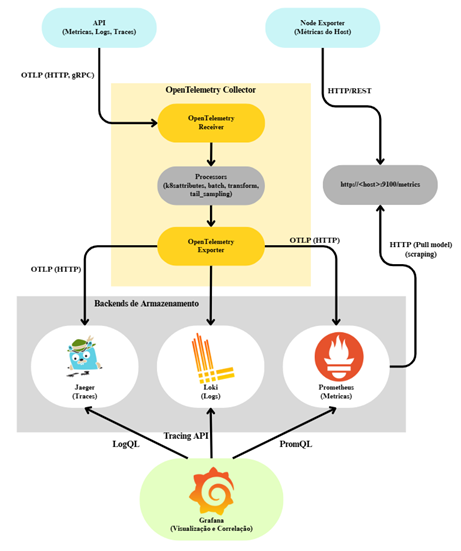
\includegraphics[width=0.8\textwidth]{images/Diagramas/arquitetura_da_solucao.png}
    \caption{Arquitetura da Solução}
    % \label{fig:digital_twin}
\end{figure}

A imagem detalha o fluxo de dados de telemetria desde a sua origem nos micros-serviços até a visualização final no Grafana. A arquitetura é composta pelas se-guintes camadas:

\begin{itemize}
    \item \textbf{APIs e SDKs} \\ As APIs (Application Programming Interfaces) definem os con-tratos para a geração e correlação de dados de telemetria. Os SDKs (Software Development Kits) são implementações específicas de linguagem das APIs, fornecendo as ferramentas necessárias para instrumentar o código das aplica-ções. Estes SDKs permitem aos utilizadores gerar dados de telemetria na sua linguagem de programação escolhida e exportá-los para um backend preferenci-al. Incluem bibliotecas de instrumentação que geram dados relevantes a partir de bibliotecas e frameworks populares (por exemplo, requisições HTTP) e dete-tores de recursos que adicionam atributos contextuais (como nome do pod ou namespace em Kubernetes) aos dados de telemetria.(OpenTelemetry Authors, 2025; \cite{Thakur2022})
    
    \item \textbf{Collector} \\ O OpenTelemetry Collector é um componente independente e agnós-tico de fornecedor, concebido para receber, processar e exportar dados de tele-metria. Atua como um hub centralizado para gerir pipelines de telemetria, rece-bendo dados em vários formatos (como OTLP, Prometheus, Jaeger) e encami-nhando-os para um ou mais backends. A sua capacidade de processar e filtrar dados antes da exportação otimiza o fluxo de dados, reduzindo a sobrecarga nas aplicações e melhorando a eficiência geral. (OpenTelemetry Authors, 2025; \cite{Thakur2022})
    
    \item \textbf{Exportadores (Exporters)} \\ Os exportadores são componentes responsáveis por enviar os dados de telemetria (após serem gerados pelas aplicações ou processa-dos pelo Collector) para ferramentas de backend específicas, como Grafana, Jaeger, Prometheus,, Loki ou outros sistemas proprietários. A utilização de ex-portadores OTLP é considerada uma boa prática, pois são concebidos para emi-tir dados OpenTelemetry sem perda de informação e são amplamente suporta-dos por diversas plataformas de observabilidade. (OpenTelemetry Authors, 2025; \cite{Thakur2022})
    
    \item \textbf{Node Exporter} \\ O Node Exporter é utilizado como agente de monitorização a nível do sistema operativo, responsável por expor métricas relacionadas com CPU, memória, disco e rede. Embora não esteja diretamente integrado no pipe-line do OpenTelemetry Collector, este componente fornece ao Prometheus da-dos cruciais sobre a infraestrutura subjacente, permitindo complementar a ob-servabilidade das aplicações com indicadores do ambiente de execução.
    
    \item \textbf{Camada de Visualização e Análise} \\ O Grafana atua como a interface de usuá-rio unificada para visualizar e analisar os dados. Ele se integra aos backends (Prometheus, Loki e Jaeger), permitindo a criação de dashboards interativos que mostram as métricas, logs e traces de maneira correlacionada.
\end{itemize}


A separação entre instrumentação (APIs e SDKs), processamento/exportação (Collector e Exportadores) e visualização confere maior flexibilidade e desacopla-mento, permitindo que as aplicações permaneçam independentes da infraestrutura de observabilidade subjacente.


\subsection{Fluxo de Telemetria}

O fluxo de dados de telemetria segue um pipeline bem definido:

\begin{enumerate}
    \item A aplicação ASP.NET Core emite dados de observabilidade (logs, métri-cas, traces) através do protocolo OTLP gRPC, e envia-os para o receiver do OpenTelemetry Collector;
    \item As métricas do sistema operativo são recolhidas diretamente pelo Promet-heus através do Node Exporter;
    \item O OTel Receiver aceita entradas de diferentes fontes, incluindo OTLP e scraping Prometheus;
    \item Os dados são então encaminhados para os processadores do Collector, que executam tarefas de transformação (transform), enriquecimento com dife-rentes atributos (attributes), agregação (batch) e amostragem de traces (tail\_sampling);
    \item Após o processamento, os dados são enviados pelo OTel Exporter para os seus respetivos destinos: Logs → Loki, Traces → Jaeger e Métricas → Prometheus;
    \item O Grafana atua como ponto de agregação visual, utilizando as linguagens de consulta específicas de cada backend para gerar dashboards interativos e correlacionados.
\end{enumerate}

\section{Detalhes Técnicos da Implementação}

\subsection{Estratégia de Instrumentação em .NET}

Do ponto de vista técnico, a instrumentação foi aplicada exclusivamente aos servi-ços criados internamente, evitando a recolha de dados de dependências externas. Desta forma, métricas, logs e traces refletem apenas o comportamento dos micro-serviços proprietários, reduzindo o ruído e a sobrecarga de dados. Esta abordagem garante que a telemetria recolhida é relevante para a análise e otimização da plata-forma, focando a monitorização nos elementos críticos sob responsabilidade direta da equipa de desenvolvimento.

A instrumentação de aplicações é um passo crucial para gerar dados de teleme-tria significativos. Em ambientes de microserviços com múltiplas APIs, a instru-mentação individual de cada serviço pode ser repetitiva e propensa a erros, para mitigar esta complexidade, foi adotada uma abordagem prática e reutilizável para a instrumentação de APIs ASP.NET Core, utilizando um pacote comum (DTX.Base.Common). Este pacote encapsula toda a configuração necessária para a emissão de traces distribuídos, métricas e logs estruturados, promovendo uma padronização e um desacoplamento eficaz entre o código da aplicação e a infraes-trutura de observabilidade.
Esta estratégia centraliza a lógica de observabilidade num único ponto, reduzin-do significativamente o código repetido. A configuração da observabilidade pode ser ativada e controlada dinamicamente através de variáveis de ambiente, o que confere grande flexibilidade e portabilidade entre diferentes ambientes (desenvol-vimento, homologação e produção). Para instrumentar novos serviços, a interven-ção é mínima: basta adicionar o pacote DTX.Base.Common, invocar um método de extensão no Program.cs e definir as variáveis de ambiente necessárias.
A lógica de observabilidade foi centralizada num único método de extensão, aplicada na inicialização de cada API .Net:

builder.ConfigureOpenTelemetry();

Este método ativa automaticamente os componentes do OpenTelemetry para instrumentação de tracing distribuído, coleta de métricas e exportação de logs es-truturados. As configurações são controladas dinamicamente por variáveis de am-biente, o que facilita a portabilidade entre diferentes ambientes, sem a necessidade de recompilação ou reconfiguração manual.

\begin{table}[H]
\centering
\caption{Variáveis de ambiente para configuração OTLP Exporter (colocar as em uso)}
\label{tab:otlp_exporter_env_vars}
\begin{tabular}{|p{6cm}|p{8cm}|}
\hline
\textbf{Variável} & \textbf{Descrição} \\
\hline
OTEL\_EXPORTER\_OTLP\_ENDPOINT & URL do collector OTLP \\
\hline
OTEL\_EXPORTER\_OTLP\_PROTOCOL & Protocolo utilizado (grpc ou http/protobuf) \\
\hline
OTEL\_EXPORTER\_OTLP\_HEADERS & Cabeçalhos opcionais no formato chave=valor (ex: Authorization=Bearer abc) \\
\hline
\end{tabular}
\end{table}


\subsection{Vantagens da Abstração da Instrumentação OpenTelemetry}

O encapsulamento da lógica de instrumentação no pacote DTx.Base.Common e a exposição via um método de extensão (ConfigureOpenTelemetry()) proporcionam benefícios significativos para o desenvolvimento e a operação de aplicações distri-buídas:

\begin{itemize}
    \item Padronização da Instrumentação entre Múltiplas APIs: Garante que todas as APIs sigam as mesmas convenções de observabilidade, resultando em dados de telemetria consistentes e facilmente comparáveis. Isso é fundamental para a cor-relação eficaz de dados em sistemas complexos;
    \item Desacoplamento da Infraestrutura de Observabilidade: O código da aplica-ção torna-se independente das ferramentas de backend utilizadas (Grafana, Jae-ger, Tempo, etc.). Se houver uma mudança nas ferramentas de observabilidade, as modificações são minimizadas e confinadas à configuração do collector ou às variáveis de ambiente, não exigindo alterações no código da aplicação;
    \item Facilidade de Configuração via Ambiente: A ativação e o ajuste da observabi-lidade são feitos através de variáveis de ambiente, o que simplifica a implanta-ção e a gestão em diferentes ambientes (desenvolvimento, homologação, produ-ção), promovendo a portabilidade;
    \item Redução Significativa de Código Repetido: Ao centralizar a lógica de obser-vabilidade num único ponto, evita-se a duplicação de código em cada novo ser-viço ou API, tornando o processo de instrumentação mais eficiente e menos propenso a erros.
\end{itemize}

Com esta abordagem, a instrumentação de novos serviços pode ser realizada com mínima intervenção, com a adição do pacote DTX.Base.Common, uma chamada simples ao método de extensão no Program.cs e a definição das variáveis de ambi-ente necessárias. Isso acelera o desenvolvimento e garante que a observabilidade seja uma parte integrante do ciclo de vida da aplicação desde o início.

\subsection{Instrumentação Específica do ASP.NET Core}

A instrumentação foi dividida nos três pilares da observabilidade, utilizando bibli-otecas de instrumentação automática para cada um.

\begin{itemize}
    \item Instrumentação de Tracing Distribuído: A instrumentação de rastrea-mento distribuído utiliza bibliotecas que monitoram requisições web, chamadas HTTP e interações com o banco de dados. Esses dados são ex-portados para o Collector.
.tracing
    .AddAspNetCoreInstrumentation()
    .AddHttpClientInstrumentation()
    .AddEntityFrameworkCoreInstrumentation()
    .AddNpgsql();
    \item Coleta de Métricas: A solução também contempla a recolha de métricas relevantes tanto ao nível da aplicação como do ambiente de execução. As métricas são coletadas pelo SDK e enviadas para o Collector.
.metrics
    .AddAspNetCoreInstrumentation()
    .AddHttpClientInstrumentation()
    .AddRuntimeInstrumentation();
    \item Logs Estruturados: A configuração de logs substitui os providers nati-vos de logging do .NET e ativa o OpenTelemetry como destino principal de logs estruturados.
builder.Logging.AddOpenTelemetry(logging =>
{
    logging.IncludeFormattedMessage = true;
    logging.IncludeScopes = true;
    logging.AddOtlpExporter();
});
\end{itemize}

A utilização de logs estruturados permite realizar pesquisas avançadas por atribu-tos, correlacionar mensagens de log com spans e traces, e visualizar os logs num contexto de execução mais rico (e.g., por serviço, requisição ou erro).

\section{Coleta de dados com o OpenTelemetry Collector}

A fase de coleta é o ponto de entrada para os dados de telemetria no pipeline de observabilidade, é responsável por capturar logs, métricas e traces gerados pelas aplicações instrumentadas, agentes sidecar ou ferramentas de terceiros. Esta coleta é feita principalmente através dos receivers do OpenTelemetry Collector, que atu-am como ouvintes ou scrapers, aceitando dados em vários formatos.
O OpenTelemetry Collector, um componente central do ecossistema, funciona como um hub de processamento centralizado, capaz de lidar com múltiplas fontes e destinos de dados, na implementação em questão, o Collector foi configurado para escutar em duas portas principais para o protocolo OTLP:
4317 para gRPC e 4318 para HTTP. Esta configuração permite que as aplica-ções enviem telemetria usando o protocolo de sua preferência, a fase de coleta é crítica para garantir que os dados cheguem de forma consistente e em tempo real ao pipeline de observabilidade.
No ambiente Kubernetes, a implantação do OpenTelemetry Collector foi reali-zada como um DaemonSet. Esta escolha de implantação garante que o Collector seja executado como um agente em cada nó (node) do cluster, em vez de ser um serviço centralizado. Cada instância do DaemonSet Collector, que age como um agente local, recebe a telemetria dos pods que estão no mesmo nó.
A principal vantagem desta abordagem é a redução de latência e a segurança. Ao coletar a telemetria localmente, os dados não precisam viajar pela rede do clus-ter, reduzindo a latência e o risco de congestionamento, além disso, essa arquitetu-ra de agente local é mais resiliente, pois a falha de um agente afeta apenas a coleta de dados de um único nó, enquanto os outros nós continuam a operar normalmen-te. Essa configuração de DaemonSet, combinada com os receivers do Collector, otimiza o fluxo de telemetria e torna-o mais robusto e eficiente

\subsection{Protocolo OTLP (gRPC/HTTP) e Configuração}

O OpenTelemetry Protocol (OTLP) é o protocolo padrão utilizado na plataforma de observabilidade para o transporte de dados de telemetria, como métricas, logs e tracing distribuído. Desenvolvido como parte do ecossistema OpenTelemetry, o OTLP é um protocolo aberto, extensível e eficiente, que permite a comunicação entre aplicações instrumentadas, agentes de coleta (como o OpenTelemetry Collec-tor) e sistemas de backend como Grafana Loki (logs), Jager (traces) e Prometheus (métricas). O protocolo suporta os formatos gRPC e HTTP/protobuf, garantindo flexibilidade de integração com diversos ambientes e ferramentas. Num cluster Kubernetes, o uso do OTLP padroniza a coleta e exportação de dados de observa-bilidade entre os pods e os componentes da infraestrutura de monitoramento, gera assim portabilidade, interoperabilidade e escalabilidade da solução implementada.

\subsection{OpenTelemetry Operator}

Gerir a observabilidade em ambientes Kubernetes pode tornar-se complexo, espe-cialmente quando é necessário configurar múltiplos Collectors, manter consistên-cia de pipelines e aplicar boas práticas de escalabilidade e segurança. Para simpli-ficar esta gestão, a comunidade desenvolveu o OpenTelemetry Operator, um Custom Kubernetes Operator que automatiza o ciclo de vida dos Collectors e a sua configuração.

\subsubsection{Conceito e Arquitetura}

O OpenTelemetry Operator expande o Kubernetes através de Custom Resource Definitions (CRDs), introduzindo novos tipos de recurso que descrevem configu-rações de observabilidade de forma declarativa.
O recurso mais importante é o OpenTelemetryCollector, no qual o utilizador defi-ne, em YAML, as características desejadas do Collector (receivers, processors, exporters e modo de execução). O Operator traduz automaticamente essa especifi-cação em objetos nativos do Kubernetes, como Deployments, DaemonSets ou ConfigMaps.

Dessa forma:

\begin{enumerate}
    \item O programador ou DevOps aplica um manifesto OpenTelemetryCollector;
    \item O Operator valida e cria os recursos Kubernetes correspondentes;
    \item O Collector é implantado de forma consistente e conforme as boas práticas de-finidas pela comunidade.
\end{enumerate}

\subsubsection{Modos de Deploy suportados}

O CRD OpenTelemetryCollector permite escolher o modo de execução do Collec-tor:

\begin{itemize}
    \item DaemonSet: cada nó do cluster executa uma instância do Collector, recolhendo telemetria localmente;
    \item Deployment: uma instância centralizada atua como gateway, agregando e ex-portando dados;
    \item Sidecar: o Collector é implantado junto de cada Pod, garantindo isolamento máximo e baixo acoplamento;
    \item StatefulSet: utilizado em cenários que exigem persistência ou configuração estável.
\end{itemize}

Essa flexibilidade permite ajustar a arquitetura de observabilidade conforme a natureza da carga de trabalho.

\subsubsection{Vantagens do Operator}

\begin{itemize}
    \item Automação: reduz a necessidade de escrever e manter manifestos Kubernetes complexos para cada Collector;
    \item Consistência: garante que todos os Collectors seguem uma configuração centra-lizada e padronizada;
    \item Integração com GitOps: por ser declarativo, integra-se facilmente em fluxos de CI/CD e ferramentas como ArgoCD ou Flux.
\end{itemize}

Evolução contínua: a comunidade mantém o Operator alinhado com novas versões do OpenTelemetry, reduzindo o risco de configuração obsoleta.

\subsection{Abordagem Adotada: DaemonSet (Agente por nodo)}

\subsubsection{Justificação da Escolha}

Optou-se por executar o OpenTelemetry Collector em DaemonSet, de forma a disponibilizar um agente local em cada nó do cluster. 

\begin{figure}[h]
    \centering
    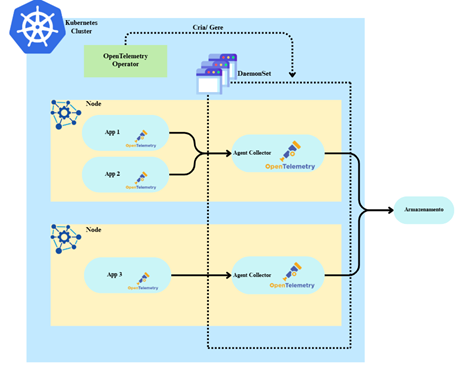
\includegraphics[width=0.8\textwidth]{images/Diagramas/daemonset_collector.png}
    \caption{Implementação de DaemonSet Collector}
    % \label{fig:digital_twin}
\end{figure}

Em cada nó, um Pod do Collector expõe receivers OTLP em gRPC (porta 4317) e HTTP/Protobuf (porta 4318), recebendo métricas, logs e traces das workloads residentes nesse nó. 

Esta opção foi guiada por três objetivos principais:  

\begin{itemize}
    \item Baixa latência na entrega de telemetria, evitando saltos de rede desnecessários antes do primeiro processamento;
    \item Resiliência local, confinando o impacto de falhas ao nó afetado; 
    \item Simplicidade de integração nas aplicações, que passam a publicar telemetria para um endpoint local único.
\end{itemize}

\subsubsection{Beneficios Observados}


A abordagem em DaemonSet resultou em menor variância de entrega dos sinais (coleta e pré-processamento locais), isolamento de falhas por nó, redução da de-pendência de rede intra-cluster e configuração simplificada do lado das aplicações (um único endpoint local, sem descoberta adicional).

\section{Processamento e Transformação dos Dados}

Após a recolha dos dados, estes passam por uma fase crítica de processamento dentro do OpenTelemetry Collector. Esta etapa, orquestrada por vários processa-dores, é essencial para modificar, enriquecer, agrupar ou filtrar os dados, garantin-do a sua compatibilidade e utilidade para os sistemas subsequentes de armazena-mento e análise.

\subsection{Processadores e as suas Aplicações}



\begin{table}[H]
\centering
\caption{Processadores Essenciais do OpenTelemetry Collector}
\label{tab:processadores_otel_collector}
\begin{tabularx}{\textwidth}{|l|X|X|X|}
\hline
\textbf{Processador} & \textbf{Função Primária} & \textbf{Aplicações-Chave} & \textbf{Significado para Observabilidade} \\
\hline
\texttt{transform} & Modifica dados de telemetria usando OTTL. & Adiciona \texttt{service.name}, converte \textit{timestamps}, normaliza severidades de \textit{logs}, aplica regras de amostragem. & Garante consistência dos dados e conformidade com convenções semânticas. \\
\hline
\texttt{batch} & Agrupa dados de telemetria em lotes. & Otimiza a exportação de dados, reduzindo chamadas de rede e sobrecargas. & Melhora o débito e a eficiência do \textit{pipeline}. Crucial para ambientes de alto volume. \\
\hline
\texttt{attributes} & Adiciona, modifica ou elimina atributos (metadados). & Injeta atributos de ambiente estáticos, enriquece com metadados do host. & Enriquece os dados com contexto crucial, melhorando a pesquisa, filtragem e correlação de dados. \\
\hline
\texttt{resource} & Modifica atributos de recurso. & Aplica consistentemente \texttt{service.name} e outros metadados fundamentais. & Assegura a uniformidade de identificadores em todos os dados de telemetria. \\
\hline
\texttt{memory\_limiter} & Previne o consumo excessivo de memória. & Protege o \textit{collector} contra falhas devido ao esgotamento de recursos. & Garante a estabilidade do \textit{pipeline}. \\
\hline
\texttt{tail\_sampling} & Amostra \textit{traces} com base no contexto completo. & Reduz o volume de dados de \textit{trace}, focando-se nos mais críticos (por exemplo, erros ou alta latência). & Otimiza custos de armazenamento e melhora o desempenho de consultas no \textit{backend}. \\
\hline
\end{tabularx}
\end{table}



\begin{itemize}
    \item{Processador transform} \\ Este processador utiliza a OpenTelemetry Transforma-tion Language (OTTL) para realizar modificações extensivas nos dados de te-lemetria. Na implementação atual, é empregado para adicionar o atributo servi-ce.name aos sinais de telemetria, converter timestamps para um formato padro-nizado, normalizar severidades de logs (por exemplo, mapeando vários níveis de log para um conjunto consistente como INFO, WARN, ERROR) e aplicar regras de amostragem dinâmicas a traces. O processador transform é fundamen-tal para garantir a consistência dos dados e a adesão a convenções semânticas predefinidas, o que é primordial para uma análise precisa e uma correlação efi-caz a jusante. Contudo, as suas poderosas capacidades exigem uma configura-ção cuidadosa para evitar "Transformações Inconsistentes" (Unsound Transfor-mations) ou "Conflitos de Identidade" (Identity Conflicts) que possam compro-meter a integridade dos dados;
    
    \item \textbf{Processador batch}  \\ Este processador agrupa eficientemente os dados de tele-metria em lotes antes de serem exportados. O batching reduz significativamente o número de chamadas de rede e a sobrecarga associada, melhorando assim o débito geral e a eficiência da exportação de dados, especialmente em ambientes de alto volume. Processador attributes: Concebido para adicionar, modificar ou eliminar atributos (metadados) em spans, logs ou métricas. Por exemplo, pode ser utilizado para injetar um atributo de ambiente estático (e.g., "produção", "desenvolvimento") em toda a telemetria de entrada ou enriquecer dados com metadados ao nível do host. Este processador é vital para enriquecer os dados de telemetria com informações contextuais cruciais, o que melhora a sua capa-cidade de pesquisa, filtragem e, em última análise, as suas capacidades de corre-lação entre diferentes sinais;
    
    \item \textbf{Processador resource} \\ Tem como alvo específico a modificação de atributos de recurso. Os atributos de recurso descrevem a entidade que produz a telemetria, como o serviço da aplicação, a máquina host ou o contentor. É crucial para ane-xar consistentemente metadados fundamentais como environment, service ver-sion ou region às métricas e para enriquecer logs com informações detalhadas de recurso. Este processador garante que atributos de identificação comuns, no-tavelmente service.name, são aplicados uniformemente em todos os sinais de te-lemetria (logs, traces e métricas). Esta consistência é fundamental para alcançar uma correlação perfeita entre sinais no Grafana;
    
    \item \textbf{Processador memory limiter} \\
    Este processador é implementado para evitar que o OpenTelemetry Collector consuma recursos de memória excessivos. Ao definir limites de memória, impede que o processo do Collector falhe devido ao esgotamento de recursos, garantindo assim a estabilidade e fiabilidade contí-nuas de todo o pipeline de observabilidade;
    
    \item \textbf{Processador tail sampling} \\ Este processador permite decisões de amostragem em traces com base no contexto completo de um trace, ou seja, depois de todos os spans relacionados com um trace terem sido recebidos. Suporta vários crité-rios de filtragem que podem ser encadeados, como amostragem baseada na latência dotrace, taxas probabilísticas, códigos de status HTTP (por exemplo, apenas traces de erro) ou limitação de taxa. A amostragem de cauda é crítica pa-ra gerir o volume de dados de trace, particularmente em sistemas distribuídos de alto tráfego. Ajuda a otimizar os custos de armazenamento e a melhorar o de-sempenho da consulta no backend de tracing sem sacrificar a capacidade de cap-turar e analisar traces críticos ou anómalos.
\end{itemize}


A capacidade do OpenTelemetry Collector de modificar todos os aspetos da tele-metria, incluindo a remoção de informações sensíveis através do processador transform, ou o enriquecimento consistente de dados com atributos específicos, posiciona-o como um ponto de controlo estratégico para a governação de dados. Esta centralização do controlo significa que os requisitos de conformidade podem ser geridos e aplicados ao nível do Collector, reduzindo a necessidade de altera-ções individuais ao nível da aplicação ou de configurações complexas específicas do backend. 
Esta abordagem centraliza significativamente o controlo de dados e minimiza a superfície de ataque para fugas acidentais de dados, além disso, a capacidade de filtrar, agrupar e reduzir a cardinalidade dos dados antes de serem exportados para o backend traduz-se diretamente em poupanças substanciais nos custos de ingestão e armazenamento de dados, especialmente para serviços de observabilidade geri-dos. Ao reduzir o volume e a complexidade dos dados na origem, o Collector me-lhora o desempenho da consulta nos backends e mitiga potenciais problemas de "Crise de Identidade" em métricas, levando a dashboards mais fiáveis. Isto torna o Collector como um componente crítico para gerir tanto a eficiência económica como operacional de toda a pilha de observabilidade.


\section{Persistência e Armazenamento de Dados }

\subsection{Armazenamento de Logs com o Loki}

O Loki foi escolhido como sistema de armazenamento de logs devido à sua arqui-tetura otimizada para consultas baseadas em etiquetas (labels) em vez de full-text search. Esta abordagem torna-o mais eficiente e menos dispendioso em termos de recursos quando comparado com soluções tradicionais, como o Elasticsearch. Os logs estruturados emitidos pelas APIs .NET são enviados ao OpenTelemetry Collector através do protocolo OTLP e, em seguida, exportados para o Loki. A integração nativa com o Grafana permite que os logs sejam visualizados e correla-cionados facilmente com métricas e traces, proporcionando uma análise unificada.

\subsection{Armazenamento de Traces com o Jaeger}

O Jaeger foi adotado como backend de armazenamento e análise de traces distri-buídos, dada a sua capacidade de oferecer visibilidade ponta a ponta sobre o ciclo de vida de uma requisição. Através da identificação do serviço (atributo servi-ce.name), é possível segmentar e filtrar os traces de forma eficaz, identificando gargalos e pontos de falha no percurso entre microserviços. Os dados são exporta-dos pelo OpenTelemetry Collector via protocolo OTLP/gRPC para o endpoint do Jaeger, onde ficam persistidos para consulta e análise detalhada no Grafana.

\subsection{Armazenamento de Métricas com o Prometheus}

O Prometheus foi selecionado como sistema de armazenamento de métricas pela sua robustez no tratamento de séries temporais e pela linguagem de consulta PromQL, que possibilita análises avançadas. As métricas da aplicação .NET são recolhidas pelo OpenTelemetry Collector e exportadas para o Prometheus, centra-lizando a coleta e evitando a exposição direta das aplicações. Complementarmente, métricas de infraestrutura provenientes do Node Exporter são recolhidas direta-mente pelo Prometheus através de scraping HTTP. Esta combinação assegura visi-bilidade tanto a nível da aplicação como da infraestrutura, permitindo uma visão abrangente do desempenho do sistema.

\chapter{Visualização e Análise de Dados}

\section{Visualização centralizada no Grafana}

A visualização dos dados de telemetria assume um papel crucial para a compreensão e monitorização eficaz de sistemas distribuídos. Embora as ferramentas Prometheus, Jaeger e Loki disponham de interfaces próprias para análise independente de métricas, \textit{traces} e \textit{logs}, a fragmentação das informações pode dificultar a correlação rápida entre estes dados. Por esse motivo, optou-se pelo Grafana como camada de visualização unificada, visando uma experiência integrada e eficiente. Entre as principais vantagens da utilização do Grafana destacam-se:

\begin{itemize}
\item A centralização das métricas, \textit{logs} e \textit{traces} num único painel interativo;
\item A capacidade avançada de correlação entre diferentes tipos de dados, facilitando a identificação de causas-raiz em anomalias;
\item A configuração unificada de alertas abrangendo todas as fontes de dados;
\item A interface intuitiva e personalizável, acessível a diferentes perfis técnicos;
\item Linguagens de consulta especializadas (\textit{PromQL}, \textit{LogQL}) diretamente integradas na ferramenta.
\end{itemize}

O Grafana habilita uma abordagem de ``\textit{single pane of glass}'', essencial para o acompanhamento consolidado do desempenho e da saúde do sistema. Além disso, permite seguir o percurso completo de uma requisição entre microsserviços e analisar a sua evolução temporal, proporcionando uma visão detalhada do comportamento distribuído da aplicação.



\break

\section{Organização dos Dashboards}

\subsection{Estrutura Lógica dos Dashboards}

Para garantir uma análise sistemática e eficiente dos dados recolhidos, a plataforma de visualização foi estruturada em diferentes painéis temáticos no Grafana. Esta organização permite um fluxo analítico claro, desde a observação de métricas de alto nível até à inspeção detalhada de eventos específicos, facilitando o diagnóstico rápido de anomalias e a compreensão do comportamento global do sistema.

De modo a assegurar uma exploração coerente e eficiente dos sinais de telemetria, os dashboards foram agrupados em três categorias principais:

\begin{itemize}
    \item \textbf{Métricas da Aplicação.} Focadas no comportamento das APIs .NET, onde são monitorizados indicadores como o número de requisições HTTP por segundo, latência média e percentis (p95 e p99), taxas de erro (4xx e 5xx), bem como o consumo de CPU e memória por serviço. Estes painéis permitem identificar padrões de carga e avaliar a eficiência operacional dos microsserviços.
    
    \item \textbf{Infraestrutura Kubernetes.} Dedicados à monitorização dos recursos do cluster, através dos dados expostos pelo Node Exporter. Incluem métricas como utilização de CPU e memória por nó e por \textit{pod}, carga média do sistema (\textit{load average}), e capacidade e utilização de armazenamento. Estes dashboards fornecem uma visão sobre a saúde da infraestrutura e permitem antecipar situações de saturação ou falhas ao nível dos recursos físicos.
    
    \item \textbf{Logs e Traces.} Concebidos para análise detalhada de eventos e interações entre serviços. Nesta secção é possível filtrar logs estruturados por nível de severidade, serviço ou mensagem, inspecionar \textit{spans} individuais e observar o encadeamento de operações entre microsserviços ao longo do tempo. Esta correlação entre logs e rastreamento distribuído suporta a identificação de pontos de falha, atrasos inesperados e comportamentos anómalos na comunicação entre componentes.
\end{itemize}

Esta estrutura modular facilita a navegação entre diferentes perspetivas operacionais e acelera o processo de diagnóstico e resolução de problemas. Para além disso, os dashboards incluem gráficos de séries temporais, indicadores numéricos e filtros dinâmicos, permitindo uma interpretação prática e contextual dos dados. Assim, a solução não apenas centraliza a telemetria, mas também proporciona aos engenheiros uma visão unificada e acionável sobre a saúde, desempenho e fiabilidade do sistema distribuído.

\subsection{Painéis de Dashboards e Metodologia de Análise}

A visualização de dados representa uma camada fundamental na estratégia de monitorização 
para sistemas distribuídos. Após a instrumentação e recolha dos sinais de telemetria, métricas, \textit{logs} e \textit{traces}, torna-se necessário disponibilizar uma interface 
capaz de sintetizar esta informação de forma clara, permitindo identificar rapidamente 
anomalias, diagnosticar problemas e interpretar o comportamento operacional das aplicações.

Nesta secção, apresentam-se os dashboards desenvolvidos no Grafana para demonstrar a 
eficácia da solução proposta. O objetivo é ilustrar o percurso analítico completo, desde 
a deteção de um evento anómalo até à identificação da sua causa, evidenciando o valor 
prático da integração entre métricas, \textit{logs} e rastreamento distribuído.

Para efeitos de consistência e clareza, os exemplos apresentados focam-se exclusivamente no 
microsserviço \textit{TicketsManagement}.

Embora fosse possível incluir visualizações de outros serviços da arquitetura, tal abordagem tenderia a revelar informações redundantes, uma vez que os padrões e métricas observados seriam aplicáveis de forma semelhante. Assim, com esta escolha conseguimos proporcionar uma análise mais clara da \textit{pipeline} de monitorização em produção, evitando a dispersão do foco e privilegiando a profundidade sobre a generalidade.

\paragraph{1) Visão geral de \textit{logs} (ponto de partida).}

A Figura~\ref{fig:dash-1} apresenta uma visão agregada de \textit{logs} estruturados emitidos pelo 
serviço \textit{TicketsManagement}. Este painel permite observar o volume total de eventos, 
distribuição por severidade e principais \textit{endpoints} envolvidos. Este é o ponto de partida do processo analítico: permite perceber rapidamente se existem picos de erros, mensagens recorrentes ou padrões anómalos.

\begin{figure}[H]
    \centering
    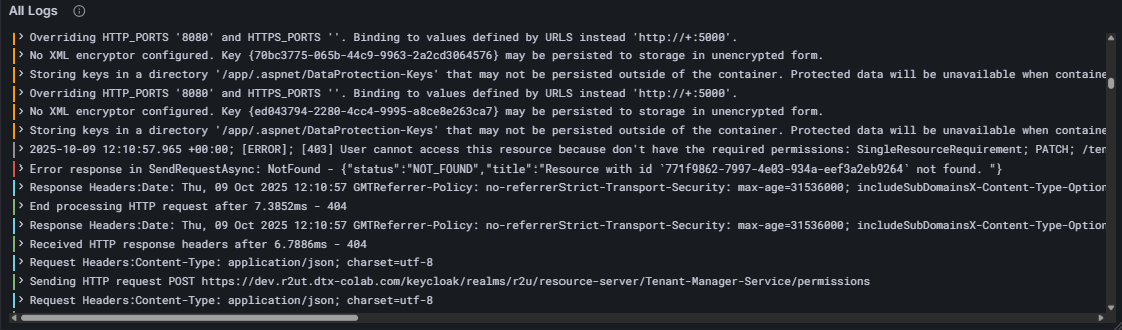
\includegraphics[width=\textwidth]{images/Grafana/all_logs_dashboard.png}
    \caption{Visão geral dos \textit{logs} estruturados do serviço \textit{TicketsManagement}.}
    \label{fig:dash-1}
\end{figure}

\textit{Transição:} Identifica-se um pico de erros ou eventos suspeitos e aplica-se filtragem 
por \texttt{service.name = TicketsManagement} e severidade (\texttt{ERROR}/\texttt{WARN}), avançando para o foco em erros.

\paragraph{2) Foco exclusivo nos erros.}

A Figura~\ref{fig:dash-2} mostra um painel dedicado exclusivamente a mensagens de erro, 
permitindo identificar \textit{endpoints} afetados, códigos HTTP e mensagens predominantes. 
Este painel acelera a identificação de falhas e reduz o \textit{MTTR} ao tornar evidentes os padrões de erro mais frequentes.

\begin{figure}[H]
    \centering
    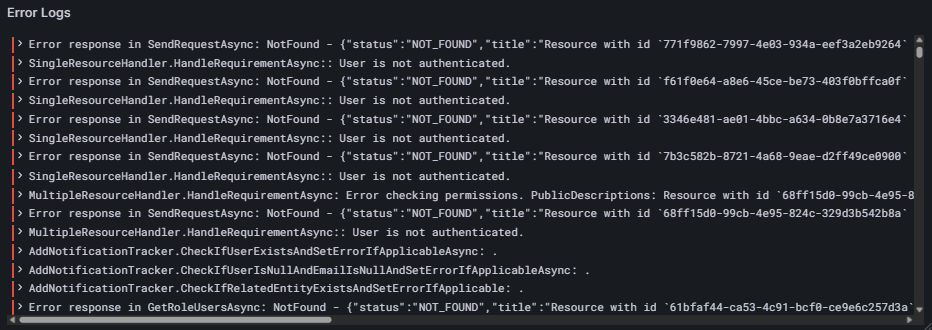
\includegraphics[width=\textwidth]{images/Grafana/error_logs_dashboard.png}
    \caption{Painel focado em \textit{logs} de erro do serviço.}
    \label{fig:dash-2}
\end{figure}

\textit{Transição:} Seleciona-se um evento concreto para análise detalhada do registo.

\paragraph{3) Expansão do registo e metadados.}

A Figura~\ref{fig:dash-3} apresenta o detalhe de um evento de \textit{log}, incluindo
\texttt{trace\_id}, \texttt{span\_id}, rota, código de estado e contexto adicional.

\begin{figure}[H]
    \centering
    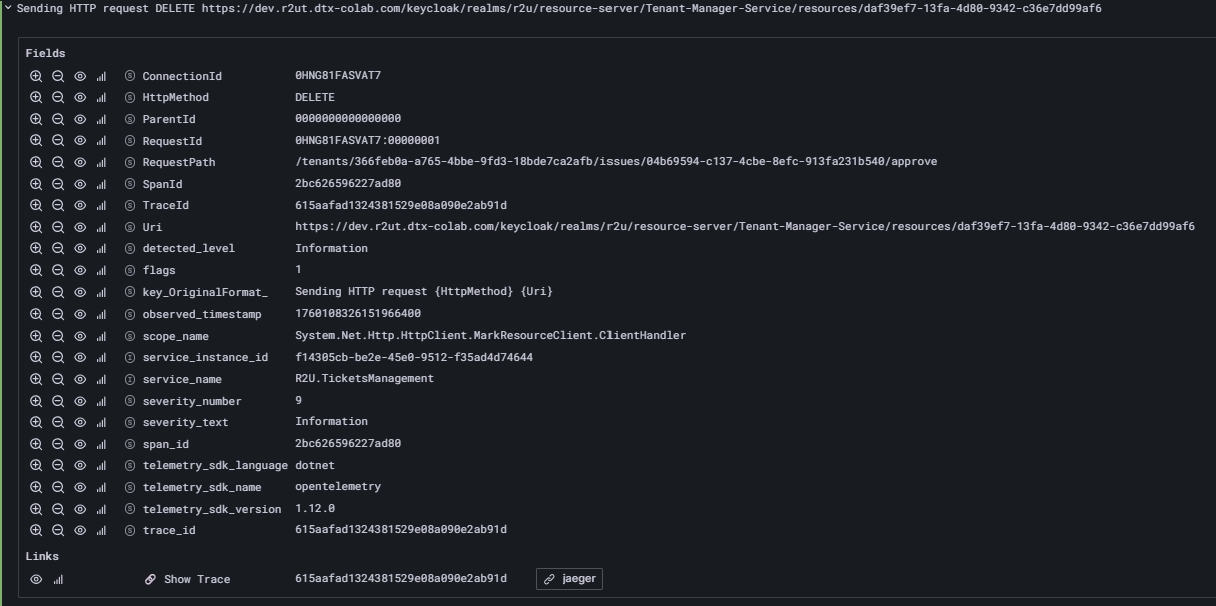
\includegraphics[width=0.9\textwidth]{images/Grafana/log_expanded.png}
    \caption{Detalhe de \textit{log} com metadados e referência direta ao trace.}
    \label{fig:dash-3}
\end{figure}

\textit{Transição:} A partir do \texttt{trace\_id}, o analista segue para o rastreamento associado.

\paragraph{4) Métricas da aplicação.}

A Figura~\ref{fig:dash-4} apresenta indicadores operacionais da API: pedidos por segundo (RPS), distribuição por códigos HTTP, latência média e percentis (p95/p99). Este painel contextualiza o erro no panorama global do serviço: variações de latência ou picos de erros tendem a refletir-se aqui.

\begin{figure}[H]
    \centering
    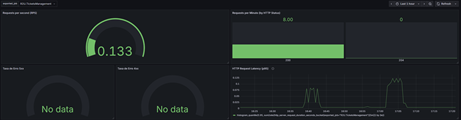
\includegraphics[width=\textwidth]{images/Grafana/metrics_dashboard.png}
    \caption{Métricas da aplicação: RPS, códigos HTTP, latência média e percentis.}
    \label{fig:dash-4}
\end{figure}

\textit{Transição.} Se houver degradação, o analista volta aos eventos e segue para o \textit{trace} para localizar gargalos. Em paralelo, valida se há limitação de recursos na infraestrutura.

\paragraph{5) Recursos da infraestrutura Kubernetes.}

A Figura~\ref{fig:dash-5} consolida métricas do cluster: utilização de CPU e memória por nó e por \textit{pod}, \textit{load average} e espaço de disco. Serve para confirmar ou excluir causas relacionadas com recursos (e.g., \textit{throttling}, saturação, \textit{out-of-memory}).

\begin{figure}[H]
    \centering
    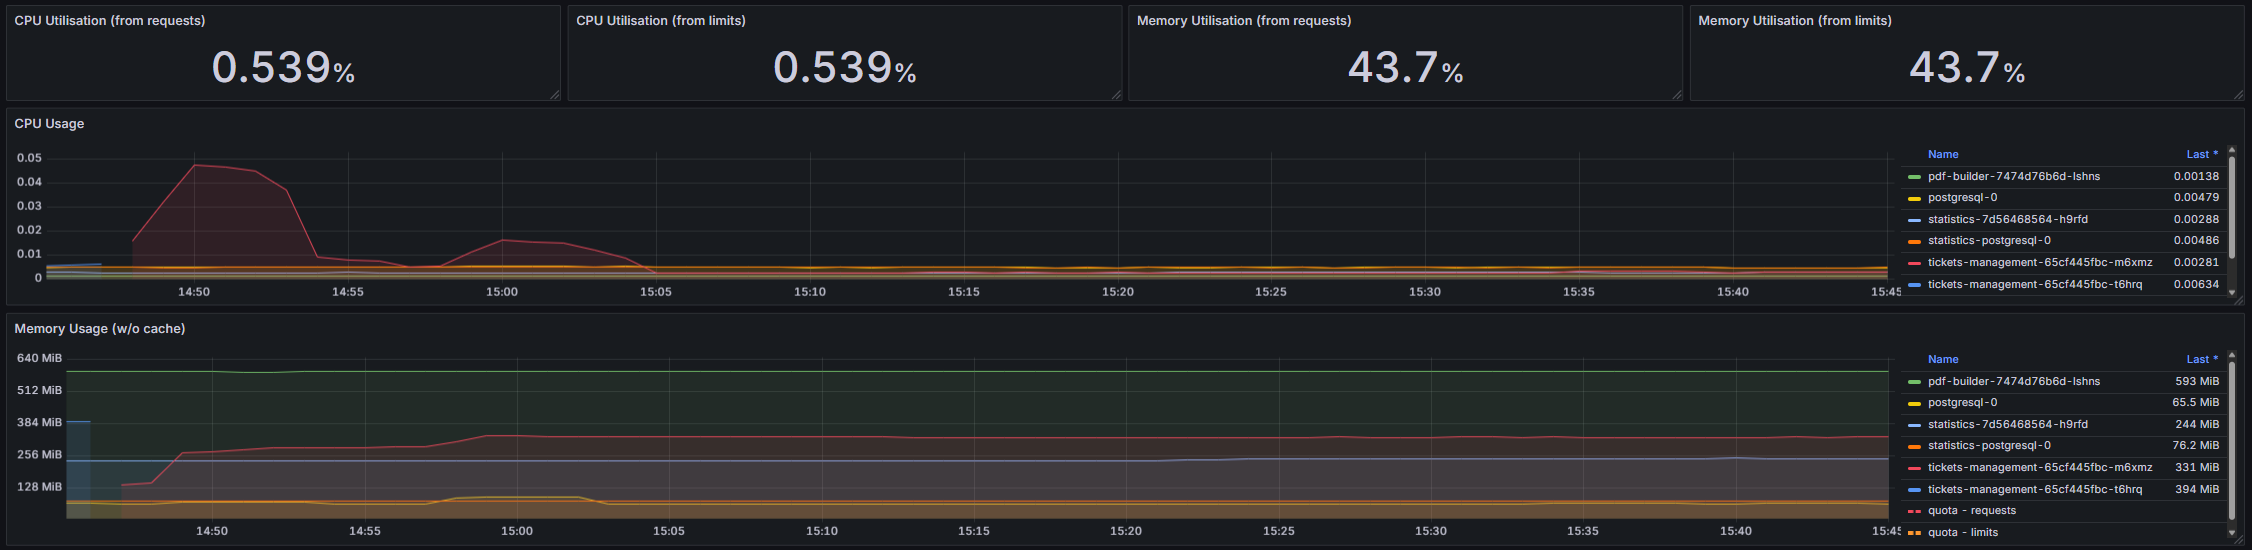
\includegraphics[width=\textwidth]{images/Grafana/cpu_memory_dashboard.png}
    \caption{Métricas de infraestrutura Kubernetes.}
    \label{fig:dash-5}
\end{figure}

 \textit{Transição.} Com os recursos estáveis, a investigação regressa ao encadeamento distribuído das chamadas para localizar a origem funcional do problema.

\paragraph{6) Rastreio distribuído.}

A Figura~\ref{fig:dash-6} ilustra um rastreamento completo associado ao incidente analisado. Observam-se as chamadas entre microsserviços, o tempo gasto em cada \textit{span} e a identificação de \textit{bottlenecks} (e.g., chamadas a \textit{databases} ou serviços externos).

\begin{figure}[H]
    \centering
    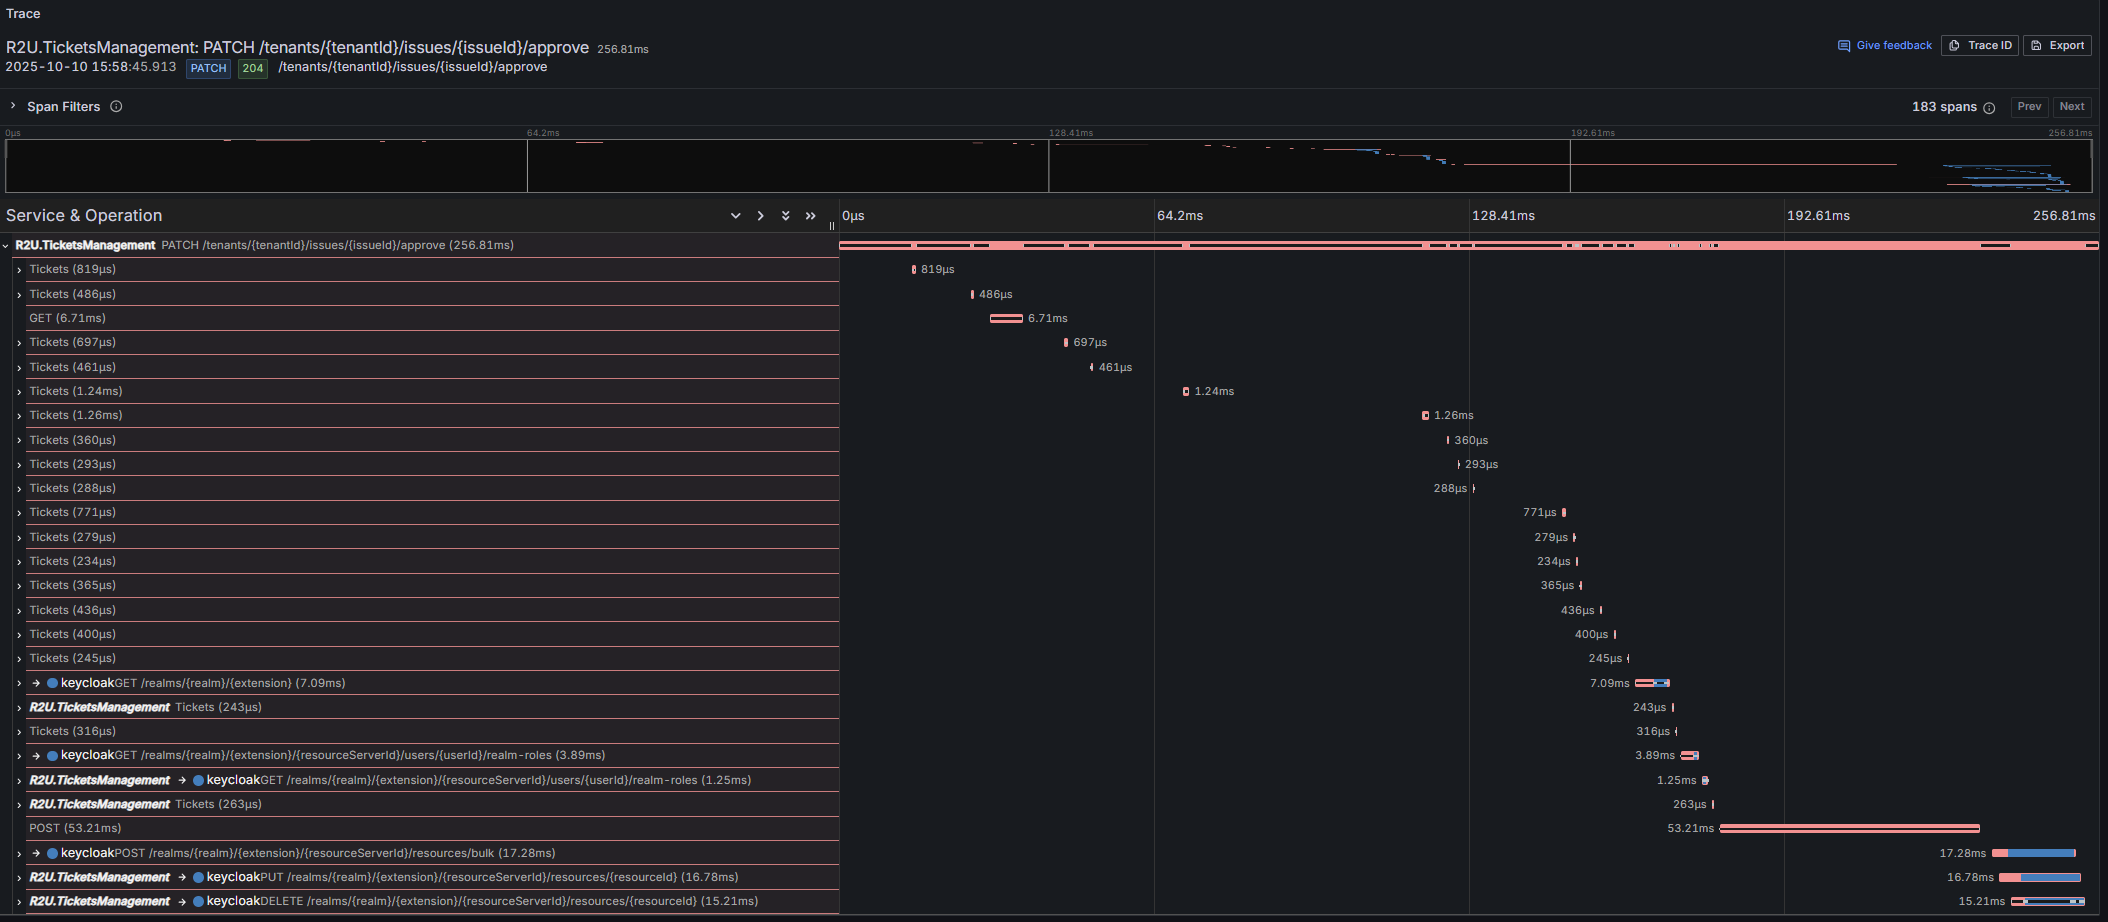
\includegraphics[width=\textwidth]{images/Grafana/trace_approve.png}
    \caption{Rastreamento distribuído associado ao evento analisado.}
    \label{fig:dash-6}
\end{figure}

\break

\subsection{Correlação entre Logs e Traces}

Um dos principais benefícios da solução implementada reside na correlação direta entre \textit{logs} 
e \textit{traces}. A Figura~\ref{fig:dash-7} apresenta um painel que liga cada registo de \textit{log} ao 
\textit{trace} correspondente, permitindo navegar rapidamente entre eventos e fluxos de execução.

\begin{figure}[H]
    \centering
    
\includegraphics[width=0.8\textwidth]{images/Grafana/trace_link_por_log.png}
    \caption{Ligação direta do \textit{log} ao \textit{trace} correspondente.}
    \label{fig:dash-7}
\end{figure}

Esta funcionalidade acelera significativamente a deteção da causa raiz de incidentes, 
uma vez que permite cruzar mensagens de erro com a linha temporal e contexto completo 
da execução distribuída.

\paragraph{Nota sobre a migração da plataforma.}
Apesar da eficácia demonstrada, importa mencionar que a plataforma R2UT encontra-se ainda 
em fase de migração gradual para Kubernetes. Assim, apenas os serviços já migrados 
emitem telemetria compatível com o modelo adotado. À medida que a migração progride, a 
monitorização será estendida a toda a plataforma, permitindo rastreamento ponta-a-ponta.

\paragraph{Síntese do fluxo analítico.}
O processo recomendado segue a sequência:

\begin{enumerate}
\item Iniciar em \textit{logs} gerais (Figura~\ref{fig:dash-1}) e identificar picos;
\item Focar erros (Figura~\ref{fig:dash-2});
\item Expandir registo e seguir o \texttt{trace\_id} (Figura~\ref{fig:dash-3});
\item Validar métricas globais (Figura~\ref{fig:dash-4});
\item Confirmar estado da infraestrutura (Figura~\ref{fig:dash-5});
\item Inspecionar \textit{trace} completo (Figura~\ref{fig:dash-6});
\item Consolidar correlação (Figura~\ref{fig:dash-7}).
\end{enumerate}

Este método reduz o tempo de análise e materializa o Grafana enquanto \textit{single pane of glass} 
para operação e diagnóstico.


\section{Alertas e Notificações Operacionais}

A monitorização eficaz não se limita à visualização passiva de métricas, exige mecanismos de alerta que permitam atuação rápida perante degradações de desempenho, falhas de serviço ou comportamentos anómalos. Para esse fim, foi configurado o \textit{Prometheus AlertManager}, responsável por receber regras de alerta definidas no Prometheus e encaminhar notificações para canais operacionais pré-definidos.

Os alertas constituem um elemento crítico em ambientes \textit{cloud-native}, onde a natureza distribuída e dinâmica dos microsserviços pode levar a falhas rápidas e efeitos em cascata. Assim, foram definidas regras de monitorização orientadas a três objetivos principais: (i) assegurar disponibilidade, (ii) detetar degradação de desempenho e (iii) prevenir saturação de recursos.

A título ilustrativo, foram implementados alertas para as seguintes condições:
\begin{itemize}
    \item Taxa de erros HTTP 5xx superior a 5\% durante 5 minutos;
    \item Latência p95 das requisições superior a 1\,s;
    \item Utilização de CPU por \textit{pod} superior a 90\% durante período prolongado.
\end{itemize}

Embora o Grafana também suporte a configuração de alertas diretamente sobre \textit{dashboards}, a opção por utilizar o \textit{AlertManager} reflete as melhores práticas para ambientes de produção, privilegiando uma abordagem declarativa, versionável e escalável. As regras de alerta podem ser geridas em ficheiros YAML, permitindo a sua integração em pipelines CI/CD e garantindo consistência operacional.

No contexto prático deste trabalho, foi integrada uma notificação para o \textit{Slack}, garantindo que as equipas técnicas recebem alertas em tempo real num canal dedicado. Esta abordagem assegura visibilidade imediata sobre incidentes operacionais e permite resposta rápida, contribuindo para a redução do \textit{Mean Time to Detect} (MTTD) e do \textit{Mean Time to Recover} (MTTR).

A Figura~\ref{fig:slack-alerts} exemplifica dois alertas gerados pelo sistema: um associado a uma taxa de erros elevada e outro à utilização excessiva de CPU num \textit{pod} Kubernetes, ilustrando a capacidade do sistema em detetar e notificar eventos críticos.

\begin{figure}[H]
    \centering
    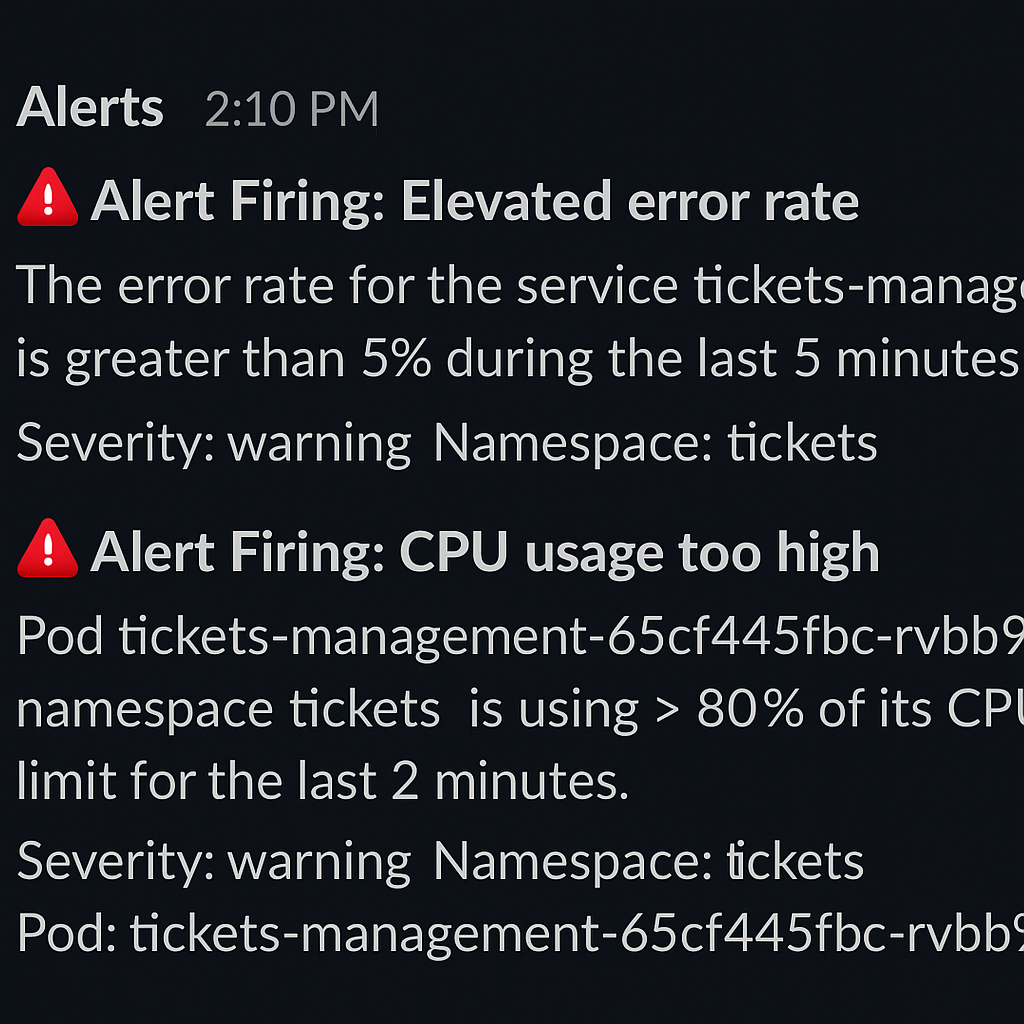
\includegraphics[width=0.5\textwidth]{images/Grafana/alertas.png}
    \caption{Notificações enviadas para o Slack contendo alertas gerados pelo \textit{AlertManager}, incluindo taxa de erros elevada e utilização excessiva de CPU.}
    \label{fig:slack-alerts}
\end{figure}



\chapter{Conclusões e Trabalho Futuro}

\section{Conclusões}

Nesta dissertação começámos por realizar uma análise crítica e aprofundada da literatura disponível sobre arquiteturas de microsserviços e sistemas de monitorização em ambientes distribuídos. Esse trabalho visou construir uma base teórica sólida que suportasse o desenvolvimento de uma plataforma de monitorização eficaz e alinhada com os objetivos do projeto R2UT, destacando-se o uso de ferramentas \textit{open-source} amplamente reconhecidas, como Prometheus, Grafana, ELK Stack e Jaeger.

A revisão bibliográfica incidiu particularmente nos desafios associados à monitorização de sistemas distribuídos dinâmicos, procurando identificar padrões de resiliência e boas práticas que assegurassem a fiabilidade, a escalabilidade e a eficiência operacional dos microsserviços. Foram igualmente aprofundados conceitos fundamentais como \textit{distributed tracing}, \textit{alerting} e observabilidade, analisando como estas técnicas podem ser combinadas para otimizar a gestão e operação de infraestruturas baseadas em microsserviços. A partir desta fundamentação teórica, foi possível estabelecer os requisitos funcionais e tecnológicos que orientaram a implementação prática.

No contexto do projeto R2UT, foi selecionado um conjunto de serviços representativos do ecossistema da plataforma, com o objetivo de demonstrar o funcionamento da solução num ambiente real e alinhado com o fluxo operacional do sistema. A escolha destes serviços permitiu validar a abordagem tomada, avaliar a capacidade de escalabilidade da solução e aferir a eficácia na deteção e investigação de falhas, garantindo simultaneamente a continuidade operacional da plataforma durante a fase de migração para Kubernetes.

A implementação de uma solução de monitorização baseada em OpenTelemetry, integrando ferramentas como Prometheus, Loki, Jaeger e Grafana, proporcionou uma visão completa e em tempo real do comportamento da aplicação distribuída. A arquitetura modular e escalável oferece flexibilidade, portabilidade e facilidade de manutenção. A correlação sinérgica entre \textit{logs}, métricas e \textit{traces}, potenciada pela padronização do OpenTelemetry, transformou a forma como a equipa de desenvolvimento e operações lida com problemas de desempenho, bem como permitiu a deteção e correção proativa de falhas e \textit{bottlenecks} no fluxo de execução dos microsserviços. A capacidade de navegar de um alerta de métrica diretamente para os \textit{traces} e \textit{logs} correspondentes em poucos segundos demonstra claramente o valor operacional desta abordagem.

Importa ainda referir que, durante o desenvolvimento, foi avaliada a adoção de \textit{zero-code instrumentation} para aplicações .NET, recorrendo a agentes automáticos de OpenTelemetry. Embora esta abordagem apresente vantagens em termos de rapidez de integração e eliminação de alterações diretas no código, verificaram-se limitações relevantes ao nível do controlo de granularidade, compatibilidade com bibliotecas utilizadas no ecossistema da aplicação e flexibilidade na definição de atributos específicos de negócio. Estas restrições levaram à opção por uma solução híbrida, baseada num pacote comum de instrumentação (\texttt{DTX.Base.Common}) e num método de extensão centralizado, garantindo simultaneamente padronização, flexibilidade e governância sobre os sinais de telemetria emitidos. Assim, a solução final alcançou um equilíbrio entre automatização e controlo fino da instrumentação, assegurando consistência técnica e alinhamento com as necessidades operacionais da plataforma.


Do ponto de vista prático, a solução revelou-se eficaz na redução do tempo médio de diagnóstico (\textit{MTTR}) e na identificação rápida de anomalias, quer ao nível da aplicação, quer ao nível da infraestrutura. Entre os principais benefícios observados destacam-se a padronização da telemetria entre serviços, a capacidade de correlação entre diferentes sinais e a redução da dependência de ferramentas proprietárias. Esta abordagem contribuiu igualmente para uma maior transparência no funcionamento interno dos serviços, permitindo apoiar decisões informadas em fases de desenvolvimento, testes e produção.

Contudo, a implementação também evidenciou desafios relevantes. A configuração inicial do \textit{pipeline} de telemetria requer conhecimento técnico especializado, nomeadamente na definição de \textit{pipelines} e recursos do OpenTelemetry Collector, de modo a evitar perdas de dados, degradação de desempenho ou consumo excessivo de memória. Adicionalmente, a instrumentação introduz algum \textit{overhead} computacional, pelo que se torna essencial aplicar boas práticas de controlo de cardinalidade, \textit{sampling} e políticas de retenção. A coexistência de múltiplos componentes \textit{open-source} com diferentes ciclos de maturidade, destacando-se a componente de \textit{logs}, que ainda depende de integrações externas como Loki ou ELK, implica um esforço contínuo de manutenção e atualização. Acresce que nem todos os serviços da plataforma R2UT se encontram ainda migrados para Kubernetes, limitando temporariamente a visibilidade transversal e a correlação total de telemetria, embora tal limitação esteja a ser mitigada pelo plano de migração progressiva em curso. Por fim, a eficácia da solução depende da literacia técnica da equipa e da adoção de processos operacionais maduros para análise e atuação sobre os indicadores de monitorização. Ainda assim, os benefícios práticos obtidos superam largamente estas limitações, demonstrando a robustez e a aplicabilidade desta abordagem em ambientes \textit{cloud-native}.

Em suma, neste trabalho conseguimos demonstrar que é possível construir um sistema de observabilidade robusto e eficiente em um ambiente \textit{cloud-native} utilizando ferramentas open-source. Essa abordagem não apenas melhora a confiabilidade e o desempenho da aplicação, mas também capacita as equipas a tomar decisões e a inovar com mais agilidade.



\section{Trabalho Futuro}

Embora a solução desenvolvida tenha demonstrado a sua eficácia na monitorização e correlação de métricas, \textit{logs} e \textit{traces} em ambiente \textit{cloud-native}, existem diversas oportunidades de evolução e consolidação que poderão potenciar significativamente o seu impacto operacional e científico.

Uma primeira linha de desenvolvimento consiste na \textbf{integração completa da telemetria em toda a plataforma R2UT}, acompanhando o plano de migração gradual para Kubernetes. A plena instrumentação de todos os serviços permitirá alcançar visibilidade ponta-a-ponta e uma correlação completa entre os fluxos de execução, tornando possível uma análise operacional verdadeiramente holística. Este esforço deverá incluir não apenas a instrumentação de novas APIs, mas também a definição de \textit{standards} internos formais para telemetria, garantindo consistência semântica e metodológica em toda a plataforma.

Outra vertente relevante consiste na \textbf{exploração da instrumentação automática (\textit{zero-code instrumentation})}, aproveitando os avanços contínuos na comunidade OpenTelemetry. Embora tenham sido identificadas limitações nesta implementação inicial, espera-se que a evolução do suporte nativo para .NET e a maturação dos agentes de instrumentação possam permitir a adoção parcial ou total desta abordagem no futuro, reduzindo o esforço de manutenção e eliminando a necessidade de inclusão de bibliotecas adicionais nos serviços.

A implementação de \textbf{dashboards avançados e automatização do \textit{alerting}} constitui também uma área de expansão crítica. A definição de \textit{Service Level Indicators} (SLI) e \textit{Service Level Objectives} (SLO) formais permitirá monitorizar níveis de serviço associados à disponibilidade, latência e fiabilidade, alinhando a observabilidade com a governança de serviço e as metas operacionais da plataforma. Complementarmente, a configuração de estratégias de alerta baseadas em anomalias e tendências (em vez de simples \textit{thresholds}) contribuirá para uma resposta mais proativa a falhas.

Outra frente de investigação com elevado potencial consiste na \textbf{integração de técnicas de Inteligência Artificial e Machine Learning} para deteção preditiva de anomalias e suporte à tomada de decisão. A análise automática de padrões de degradação e a implementação de mecanismos de correlação assistida poderão reduzir tempos de diagnóstico, potenciar respostas automáticas e aproximar a plataforma de um modelo de operação AIOps.

A adoção de mecanismos de \textbf{tracing unificado em ambientes híbridos e de múltiplos clusters} representa também um caminho promissor, possibilitando a observação integrada de componentes que residam em infraestruturas distintas (por exemplo, máquinas físicas, serviços externos e múltiplos clusters Kubernetes). Esta abordagem pode ser suportada por \textit{OpenTelemetry Gateways}, arquiteturas \textit{mesh} de observabilidade e mecanismos de encriptação e roteamento seguro de telemetria.

Por fim, uma linha de evolução natural reside na \textbf{automação do ciclo de vida da observabilidade com práticas GitOps}, garantindo que configurações do OpenTelemetry Collector, dashboards Grafana e regras de alerta são versionadas, auditáveis e sincronizadas com o estado desejado do cluster. Tal abordagem reforçará a consistência, segurança e fiabilidade do sistema ao longo do tempo.

Em suma, o trabalho futuro deverá focar-se na expansão da cobertura, no aumento do grau de automação, na integração de capacidades inteligentes e na consolidação de práticas de observabilidade como parte integrante do ciclo de vida de desenvolvimento e operação da plataforma. Ao perseguir estas linhas de evolução, será possível não só ampliar o valor prático desta solução no contexto do R2UT, como também contribuir para o avanço do estado da arte em observabilidade aplicada a sistemas distribuídos e ambientes industriais.


\renewcommand{\baselinestretch}{1}
\bibliographystyle{plainnat}
\bibliography{dissertation}
\printindex

% \appendix
% \renewcommand\chaptername{Apêndice}

% \part{Apêndices}

% \input{appendices/SupportWork}
% \chapter{Details of results}

\section{Example JSON body for creation of device via API}
\label{appendix:example}
\begin{verbatim}
  {
  "policyId": "org.eclipse ditto:577247a5-1438-48d5-b485-d41f673cac61",
  "definition": "com.smarttech:thermostat:1.0.0",
  "attributes": {
    "manufacturer": "SmartTech Solutions",
    "location": "New York, Office 2A",
    "serialno": "T10039284",
    "model": "ThermoX Pro 2000"
  },
  "features": {
    "temperature-control": {
      "definition": [
        "com.smarttech:thermostat:1.0.0"
      ],
      "properties": {
        "currentTemperature": 22.5,
        "targetTemperature": 24,
        "mode": "heating"
      }
    },
    "humidity-sensor": {
      "properties": {
        "configuration": {
          "samplingRateSeconds": 60,
          "thresholdAlert": 70
        },
        "status": {
          "humidityLevel": 45,
          "lastUpdated": "2025-06-24T10:00:00Z"
        }
      }
    }
  }
}
\end{verbatim}

\section{Thermostat DBIRTH payload in MQTT}
\label{appendix:details-of-resultsdbirth}
\begin{verbatim}
{
  "timestamp": {
    "low": -1719890226,
    "high": 408,
    "unsigned": true
  },
  "metrics": [
    {
      "name": "Temperature",
      "alias": {
        "low": 1,
        "high": 0,
        "unsigned": true
      },
      "timestamp": {
        "low": -1719890226,
        "high": 408,
        "unsigned": true
      },
      "datatype": 10,
      "isNull": true,
      "properties": {
        "keys": [
          "engUnits",
          "permission"
        ],
        "values": [
          {
            "type": 12,
            "stringValue": "inHg"
          },
          {
            "type": 12,
            "stringValue": "read-write"
          }
        ]
      }
    },
    {
      "name": "Device Control/Rebirth",
      "alias": {
        "low": 2,
        "high": 0,
        "unsigned": true
      },
      "timestamp": {
        "low": -1719890226,
        "high": 408,
        "unsigned": true
      },
      "datatype": 11,
      "isNull": true,
      "properties": {
        "keys": [
          "engUnits",
          "permission"
        ],
        "values": [
          {
            "type": 12,
            "stringValue": "inHg"
          },
          {
            "type": 12,
            "stringValue": "read-write"
          }
        ]
      }
    }
  ],
  "seq": {
    "low": 14,
    "high": 0,
    "unsigned": true
  }
}
\end{verbatim}

\section{Thermostat payload in MQTT for DDATA}
\label{appendix:details-of-resultsddata}
\begin{verbatim}
{
  "timestamp": {
    "low": -1719847593,
    "high": 408,
    "unsigned": true
  },
  "metrics": [
    {
      "alias": {
        "low": 1,
        "high": 0,
        "unsigned": true
      },
      "timestamp": {
        "low": -1719847593,
        "high": 408,
        "unsigned": true
      },
      "datatype": 10,
      "properties": {
        "keys": [
          "engUnits"
        ],
        "values": [
          {
            "type": 12,
            "stringValue": "inHg"
          }
        ]
      },
      "doubleValue": 3.2944017837137736
    },
    {
      "alias": {
        "low": 2,
        "high": 0,
        "unsigned": true
      },
      "timestamp": {
        "low": -1719847593,
        "high": 408,
        "unsigned": true
      },
      "datatype": 11,
      "properties": {
        "keys": [
          "engUnits"
        ],
        "values": [
          {
            "type": 12,
            "stringValue": "inHg"
          }
        ]
      },
      "booleanValue": false
    }
  ],
  "seq": {
    "low": 15,
    "high": 0,
    "unsigned": true
  }
}
\end{verbatim}

% \input{appendices/Listings}
% \input{appendices/Tooling}

\pagestyle{empty}
\cleartoevenpage
\null
\thispagestyle{empty}
\pagecolor{PANTONECoolGray7C}
\afterpage{\nopagecolor}
\newpage

\begin{backcover}
\thispagestyle{empty}{~\vfill
\noindent
\vfill ~}
\end{backcover}



\end{document}
